% fifo_sizing_analytical.tex -- generated from scripts/fifo_sizing_analytical.tex.in
% by scripts/build_tex.py (the code listings are copied verbatim from the
% source tree); edit the .tex.in, not this file.
\documentclass[10pt,a4paper]{article}
\usepackage[T1]{fontenc}
\usepackage[utf8]{inputenc}
\usepackage{lmodern}
\usepackage[margin=2.2cm]{geometry}
\usepackage{amsmath,amssymb}
\usepackage{booktabs}
\usepackage{array}
\usepackage{xcolor}
\usepackage{listings}
\usepackage{tikz}
\usetikzlibrary{arrows.meta,positioning,calc}
\usepackage{pgfplots}
\pgfplotsset{compat=1.16}
\usepackage[hidelinks]{hyperref}

\lstset{
  language=Python,
  basicstyle=\ttfamily\scriptsize,
  numbers=left,
  numberstyle=\tiny\color{gray},
  numbersep=6pt,
  keywordstyle=\color{blue!60!black}\bfseries,
  commentstyle=\color{green!40!black},
  stringstyle=\color{red!50!black},
  showstringspaces=false,
  columns=fixed,
  keepspaces=true,
  breaklines=true,
  breakatwhitespace=false,
  frame=single,
  framerule=0.3pt,
  rulecolor=\color{gray!60},
  xleftmargin=2.2em,
  framexleftmargin=1.8em,
  aboveskip=6pt,
  belowskip=6pt,
  tabsize=4,
}

\newcommand{\code}[1]{\texttt{#1}}
\newcommand{\Tg}{T}           % global period
\newcommand{\Tp}{T_{\mathrm{p}}} % pacer threshold
\newcommand{\NF}{N}            % tokens per frame
\newcommand{\file}{\code{derive\_characteristic.py}}

\title{Analytical FIFO sizing in FINN:\\ from token access vectors to FIFO depths}
\author{Documentation of branch \code{feature/dev/analytical-fifo-sizing}, commit \code{4ce1bd188}}
\date{}

\begin{document}
\maketitle

\begin{abstract}
FINN's \code{heuristic\_analytical} and \code{heuristic\_rtlsim} FIFO-sizing
strategies first give every dataflow node a \emph{token access vector} (TAV), a
per-cycle record of when it reads and writes stream words, and then derive all
FIFO depths from those vectors without simulating the stitched design. This
document explains the second half: how the TAVs are turned into a wall-clock
\emph{schedule} of every edge, which \emph{passes} are run over that schedule and
how their results are combined, and every \emph{rule} that changes a depth. Each
step is shown on the real code (verbatim excerpts with file and line numbers)
and on small graphs whose numbers were produced by running the code (scripts in
\code{scripts/}, Appendix~\ref{app:repro}).
\end{abstract}

\tableofcontents

%======================================================================
\section{Scope, flow and notation}
%======================================================================

Unless noted otherwise, all code is in
\code{src/finn/transformation/fpgadataflow/derive\_characteristic.py} (``\file''
below). The builder step \code{step\_set\_fifo\_depths} runs the heuristic strategies as follows:

\begin{lstlisting}[firstnumber=1097,title={\texttt{src/finn/builder/build\_dataflow\_steps.py}, lines 1097--1131}]
        elif strategy in ("heuristic_analytical", "heuristic_rtlsim"):
            # Heuristic FIFO sizing from per-node token access vectors. The two
            # strategies share everything below and differ only in tav_strategy,
            # i.e. whether a node's schedule comes from its tree model or rtlsim.
            model = model.transform(InsertDWC())
            model = model.transform(SpecializeLayers(cfg._resolve_fpga_part()))
            model = model.transform(GiveUniqueNodeNames())
            model = model.transform(AnnotateCycles())

            # heuristic_analytical takes each node's schedule from its tree
            # model, so only the nodes without one need IP generated for rtlsim
            only_jit_nodes_without_tree = tav_strategy == "tree_model"

            model = model.transform(
                JustInTimeSynthesize(
                    cfg._resolve_fpga_part(),
                    cfg._resolve_hls_clk_period(),
                    only_jit_nodes_without_tree,
                )
            )
            period = int(model.analysis(dataflow_performance)["max_cycles"])
            model = model.transform(
                DeriveTokenAccessVectors(
                    model,
                    period,
                    tav_strategy,
                    cfg._resolve_fpga_part(),
                    cfg._resolve_hls_clk_period(),
                )
            )

            period = int(
                model.analysis(partial(dataflow_performance, use_characterized=True))["max_cycles"]
            )
            model = model.transform(DeriveFIFOSizes(period=period))
\end{lstlisting}

Width converters are inserted (\code{InsertDWC}) and every node is specialized
\emph{before} characterization, so DWCs are ordinary characterized nodes
(Section~\ref{sec:dwc}). \code{DeriveTokenAccessVectors} writes the TAVs into the
node attributes \code{io\_chrc\_in}/\code{io\_chrc\_out} (from the node's tree
model for \code{heuristic\_analytical}, from a single-node rtlsim for
\code{heuristic\_rtlsim}); nothing afterwards modifies a TAV. The period handed to
\code{DeriveFIFOSizes} is the largest TAV period
(\code{dataflow\_performance(use\_characterized=True)}). \code{DeriveFIFOSizes}
writes \code{inFIFODepths}/\code{outFIFODepths}, from which \code{InsertFIFO}
creates the FIFOs. Everything in this document happens inside
\code{DeriveFIFOSizes}.

\paragraph{What a TAV is.} For a node characterized over two back-to-back frames
of $P$ cycles each, a TAV row is an integer array $c[0..2P-1]$: $c[i]$ is the
number of tokens (stream words, i.e.\ one transfer of the stream at its folded
width, not bits) transferred on that stream up to and including local cycle
$i$, assuming the node is never stalled. There is one row per stream for rtlsim
TAVs, one row per direction for tree-model TAVs. $P = \mathrm{len}(c)/2$ is the
node's \emph{period}. The TAV is a schedule on the node's \emph{local} clock and has an
arbitrary phase: local cycle 0 need not be the start of a frame.

\paragraph{Notation.}
\begin{center}
\begin{tabular}{@{}ll@{}}
\toprule
$P_v$ & period of node $v$: half its TAV length (\code{node\_periods}) \\
$\Tg$ & global period: $\max(\text{caller's period}, \max_v P_v)$, the frame interval of the graph\\
$\Tp$ & pacer threshold $0.995\,\Tg$ (\code{PACER\_TOLERANCE}); a node with $P_v\ge\Tp$ is a \emph{pacer}\\
$\NF$ & tokens per frame on an edge (\code{Edge.per\_frame}: the producer's first-frame writes)\\
$w_k$, $r_k$ & wall-clock cycle at which token $k$ of an edge is written / read ($k=1..2\NF$)\\
$t_{\mathrm{up}}, t_{\mathrm{prop}}, t_{\mathrm{full}}$ & chain periods carried with an edge (Section~\ref{sec:chain})\\
\bottomrule
\end{tabular}
\end{center}

\paragraph{The examples.} Toy graphs are chains or residual blocks of real FINN
HW nodes (\code{MVAU\_hls}/\code{MVAU\_rtl}, \code{DuplicateStreams\_hls},
\code{ElementwiseAdd\_hls}) built with the helpers of
\code{tests/fpgadataflow/test\_fifosizing\_chained\_tav.py}, renamed to role names
(A, B, C, P, X, \dots) and given \emph{hand-made} TAVs of 8 tokens a frame so
that complete schedules fit in a table (\code{fifotrace.inject} stores them
exactly as the tree-model path does). The unit-test graphs themselves, with
their tree-model TAVs, are used as well (U1--U6), and E11 is the
\code{StreamingConcat} graph of \code{test\_join\_window\_floor\_concat} (fork,
\code{FMPadding}, \code{ConvolutionInputGenerator\_rtl}, concat), which needs no TAV. In a toy TAV, ``reads at
cycles $0,2,\dots,14$, $P=16$'' means one token at each listed cycle of each of
the two frames. Every number below is printed by
\code{scripts/fifo\_examples.py}; the full output is
\code{scripts/fifo\_examples\_output.txt}. The tracer \code{scripts/fifotrace.py} only wraps the
module's functions and re-derives the intermediate terms of \code{edge\_depth},
asserting that they reproduce the depth the code returned.

%======================================================================
\section{Overview of \code{DeriveFIFOSizes}}\label{sec:overview}
%======================================================================

\begin{enumerate}
\item Run the \emph{chained-TAV pass} \code{derive\_chained\_tav\_depths} four times,
  for $(\text{causal},\text{latency})\in\{0,1\}^2$, and keep the largest depth of
  each edge (Section~\ref{sec:passes}).
\item Raise every input of a two-stream join or of a \code{StreamingConcat} to its
  \emph{join window floor} (\code{join\_window\_floors}, Section~\ref{sec:joinfloor}).
\item Write the depths: at least 2 on every edge, \code{io\_fifo\_depth} (5) on the graph
  input and output (Section~\ref{sec:write}).
\end{enumerate}

\begin{lstlisting}[firstnumber=1181,title={\texttt{src/finn/transformation/fpgadataflow/derive\_characteristic.py}, lines 1181--1200}]
    def apply(self, model):
        # Derivations of the same requirement, differing in whether a node's
        # first-frame writes are held to the inputs that carry them
        # (``causal_writes``) and in whether nodes have a pipeline latency.
        # Without the hold a producer's run-ahead survives; with it a compacting
        # node shows its real latency. The latency lengthens the slower path
        # into a join, but can also smooth a pacer's read bursts. Each is a
        # lower bound, so the largest is taken per edge.
        depths = {}
        for causal in (False, True):
            for latency in (False, True):
                found = derive_chained_tav_depths(model, self.period, causal, latency)
                for tensor, depth in found.items():
                    if depth > depths.get(tensor, 0):
                        depths[tensor] = depth
        # no join input below what the fork has to write before the join can start
        hw_nodes = [n for n in model.graph.node if is_hls_node(n) or is_rtl_node(n)]
        for tensor, depth in join_window_floors(model, hw_nodes, self.period).items():
            if depth > depths.get(tensor, 0):
                depths[tensor] = depth
\end{lstlisting}

One chained pass (Sections~\ref{sec:prep}--\ref{sec:rules}) is:
\begin{enumerate}
\item read every TAV and bind its rows to tensors (\code{read\_node\_tavs}, \code{stream\_curves});
\item compute the periods, $\Tg$, the pacer drivers and the reconvergent-branch nodes;
\item visit the nodes in graph (topological) order; for each node map its local clock to
  wall-clock time given the write times of its inputs (\code{local\_clock}), place its reads
  and writes on the wall clock (\code{token\_times}), modify the writes by the causal and
  latency rules, and store an \code{Edge} record per output;
\item for every input edge of the node, compute the steady-state peak occupancy
  (\code{peak\_occupancy}) and turn it into a depth (\code{edge\_depth}).
\end{enumerate}

%======================================================================
\section{Preparation: TAV binding, periods, pacers, branches}\label{sec:prep}
%======================================================================

\subsection{Binding TAV rows to tensors}

\begin{lstlisting}[firstnumber=260,title={\texttt{src/finn/transformation/fpgadataflow/derive\_characteristic.py}, lines 260--286}]
def stream_curves(node, inst, rows_in, rows_out):
    """Bind TAV rows to tensor names: ``({tensor: curve}, {tensor: curve})``.

    The per-stream binding is only taken when the row count matches the stream
    count, which is the shape rtlsim produces. Otherwise (tree models) row 0 is
    used for every stream.
    """
    in_curves, out_curves = {}, {}
    if rows_in is not None:
        streamed = []
        for i, t in enumerate(node.input):
            try:
                if inst.get_instream_width(i) == 0:
                    continue
            except Exception:
                pass
            streamed.append(t)
        if len(streamed) == rows_in.shape[0]:
            in_curves = {t: rows_in[k] for k, t in enumerate(streamed)}
        else:
            in_curves = {t: rows_in[0] for t in node.input}
    if rows_out is not None:
        if len(node.output) == rows_out.shape[0]:
            out_curves = {t: rows_out[k] for k, t in enumerate(node.output)}
        else:
            out_curves = {t: rows_out[0] for t in node.output}
    return in_curves, out_curves
\end{lstlisting}

Streams of width 0 (embedded weights/thresholds) are skipped. If the number of
rows equals the number of streams (rtlsim), each tensor gets its own row;
otherwise (tree models, one row) row~0 is used for \emph{every} input, including
a decoupled weight stream---those are later ignored because no edge schedule
exists for them (line 970 below). \code{read\_node\_tavs} stores, per node, row~0 of
the input and output TAV (\code{tin}, \code{tout}) and these per-tensor curves; a
node whose TAV cannot be read gets \code{(None, None, \{\}, \{\})} and is treated
like a fork/join (transparent). Forks (\code{DuplicateStreams}), joins
(\code{AddStreams}, \code{ElementwiseAdd} with two streamed inputs) and FIFOs are
never characterized (\code{\_UNCHARACTERIZED\_OPS}, \code{is\_stream\_join}).

\subsection{Periods, global period, pacers}

\begin{lstlisting}[firstnumber=626,title={\texttt{src/finn/transformation/fpgadataflow/derive\_characteristic.py}, lines 626--659}]
def node_periods(nodes, tavs):
    """Step 2: each node's own period, half its TAV length. Forks and joins
    have no TAV and no period of their own."""
    return {n.name: len(tavs[n.name][0]) // 2 for n in nodes if tavs[n.name][0] is not None}


def pacer_drivers(model, nodes, own_period, pacer_period):
    """Step 3: ``{node name: bool}``, True if the node runs at the pacer's
    period or feeds something that does. A consumer for which this is False
    can be throttled: it finishes its frame later without slowing the graph."""
    drives_pacer = {}
    for node in reversed(nodes):
        below = any(
            drives_pacer.get(cons.name)
            for cons in (model.find_consumer(t) for t in node.output)
            if cons is not None
        )
        drives_pacer[node.name] = own_period.get(node.name, 0) >= pacer_period or below
    return drives_pacer


def downstream_periods(model, nodes, own_period):
    """``{node name: period}``: the slowest own period of the node and of
    everything below it. A stall of the node delays all of them; the slack the
    slowest one has left bounds how long the node may wait."""
    slowest = {}
    for node in reversed(nodes):
        below = [
            slowest.get(cons.name, 0)
            for cons in (model.find_consumer(t) for t in node.output)
            if cons is not None
        ]
        slowest[node.name] = max([own_period.get(node.name, 0)] + below)
    return slowest
\end{lstlisting}
\begin{lstlisting}[firstnumber=870,title={\texttt{src/finn/transformation/fpgadataflow/derive\_characteristic.py}, lines 870--881}]
    nodes = [n for n in model.graph.node if is_hls_node(n) or is_rtl_node(n)]
    tavs = read_node_tavs(model, nodes)
    own_period = node_periods(nodes, tavs)

    # Global period: the slower of the caller's estimate and the slowest
    # measured TAV period (some ops' cycle estimates under-state their period).
    global_period = max(int(global_period or 0), max(own_period.values(), default=0), 1)
    pacer_period = global_period * PACER_TOLERANCE
    drives_pacer = pacer_drivers(model, nodes, own_period, pacer_period)
    t_down = downstream_periods(model, nodes, own_period)
    in_branch = reconvergent_branch_nodes(model, nodes)
    graph_inputs = {x.name for x in model.graph.input}
\end{lstlisting}

$P_v=\mathrm{len}(\code{tin})/2$. $\Tg$ is the larger of the caller's period and the
slowest TAV (the builder passes the slowest TAV period, so the two agree there;
the $\max$ protects \code{DeriveFIFOSizes(period=None)} and under-estimated
cycle counts). \code{pacer\_drivers} walks the nodes in reverse order: a node
\emph{drives the pacer} if it is a pacer ($P_v \ge \Tp$) or any consumer of its
outputs drives the pacer. A consumer that does not drive the pacer is
\emph{throttleable}: it may finish its frame later without slowing the graph,
because nothing downstream of it runs at $\Tg$. Forks and joins have period 0 and
drive the pacer only through their consumers. Because of the tolerance
$\Tp=0.995\Tg$, a bottleneck that is several nodes wide with periods a few cycles
apart is treated as one pacer (rule R4b). \code{downstream\_periods}, in the same
reverse walk, records for every node the slowest own period of the node and of
everything below it; for an edge's consumer this is $t_{\mathrm{below}}$ of the
throttled cap and the decoupled chain (R7, R7b).

\subsection{Reconvergent branches}

\begin{lstlisting}[firstnumber=662,title={\texttt{src/finn/transformation/fpgadataflow/derive\_characteristic.py}, lines 662--689}]
def reconvergent_branch_nodes(model, nodes):
    """Step 4: the nodes between a fork and the node its branches reconverge
    at. Their deadline is the join, not the frame, so their edges are never
    relaxed (``fill_only`` below)."""

    def reachable(tensor):
        seen, stack = set(), [model.find_consumer(tensor)]
        while stack:
            n = stack.pop()
            if n is None or n.name in seen:
                continue
            seen.add(n.name)
            for t in n.output:
                stack.append(model.find_consumer(t))
        return seen

    in_branch = set()
    for node in nodes:
        outs = [t for t in node.output if model.find_consumer(t) is not None]
        if len(outs) < 2:
            continue
        reach = [reachable(t) for t in outs]
        shared = set.intersection(*reach)
        if not shared:
            continue  # the branches never meet again; ordinary chains
        for r in reach:
            in_branch |= r - shared
    return in_branch
\end{lstlisting}

For every node with two or more consumed outputs (a fork), the sets of nodes
reachable from each output are intersected; the nodes reachable from some but not
all outputs lie on a branch between the fork and the node where the branches
reconverge. Their input edges, and every input edge of a node with more than one
produced input (a join, a dynamic MVAU), are \code{fill\_only} (lines 936--937):
their deadline is the join, not the frame, and they are never relaxed (rule R8).

%======================================================================
\section{The schedule}\label{sec:schedule}
%======================================================================

\subsection{Time base, frames, periods}

All times are integer clock cycles of one wall clock shared by the whole graph.
The schedule covers exactly the two frames stored in the TAVs: every edge gets
$2\NF$ write times $w_1\le\dots\le w_{2\NF}$ and $2\NF$ read times. Frames are not
simulated beyond that; steady state is obtained analytically by assuming that the
frame schedule repeats every $\Tg$ cycles (\code{periodic\_peak},
Section~\ref{sec:peak}). There is no global ``cycle 0 of the frame'': the time
origin is the moment the graph input starts; every node's offset follows from the
max-plus recurrence below. Since a TAV has an arbitrary phase, a node's first write
minus first read is \emph{not} its latency; rules R11--R13 correct for this.

\subsection{Paced graph input (rule R1)}

\begin{lstlisting}[firstnumber=692,title={\texttt{src/finn/transformation/fpgadataflow/derive\_characteristic.py}, lines 692--697}]
def graph_input_schedule(curve, global_period):
    """Write times of the tokens on a graph input: one frame per
    ``global_period``, evenly spaced. Without this the source is infinitely
    fast and every edge above the bottleneck grows without bound."""
    rate = global_period / max(int(curve[len(curve) // 2 - 1]), 1)
    return (np.arange(1, int(curve[-1]) + 1) * rate).astype(np.int64)
\end{lstlisting}

The graph input delivers the $\NF$ tokens of a frame evenly over $\Tg$ cycles:
token $i$ ($1$-based) at $\lfloor i\,\Tg/\NF\rfloor$, for both frames. $\NF$ is
the first node's per-frame reads (\code{curve[len//2-1]}).

\subsection{Local clock: the max-plus recurrence}

\begin{lstlisting}[firstnumber=294,title={\texttt{src/finn/transformation/fpgadataflow/derive\_characteristic.py}, lines 294--303}]
def arrival_of(schedule, counts):
    """Time at which ``counts[i]`` tokens have arrived, given per-token times.

    Counts beyond the schedule are clipped to its last token. An empty schedule
    constrains nothing, so every arrival time is 0.
    """
    if len(schedule) == 0:
        return np.zeros(len(counts), dtype=np.int64)
    idx = np.clip(counts, 0, len(schedule)) - 1
    return np.where(counts > 0, schedule[np.maximum(idx, 0)], 0)
\end{lstlisting}
\begin{lstlisting}[firstnumber=700,title={\texttt{src/finn/transformation/fpgadataflow/derive\_characteristic.py}, lines 700--725}]
def local_clock(span, in_scheds):
    """Wall-clock time of each local cycle of a node, given ``{tensor:
    (write times, curve)}`` for its streamed inputs: the max-plus recurrence

        R(c) = max(R(c - 1) + 1, arrival time of the tokens read by cycle c)

    as a running maximum of ``req(c) - c``. A node stalls exactly as long as
    its latest input is late."""
    cycles = np.arange(span, dtype=np.int64)
    req = np.zeros(span, dtype=np.int64)
    for sched, curve in in_scheds.values():
        req = np.maximum(req, arrival_of(sched, curve))
    return cycles + np.maximum.accumulate(req - cycles)


def token_times(clock, curve):
    """Wall-clock time of each token of ``curve`` (a cumulative count per local
    cycle) on a node whose local cycles happen at ``clock``."""
    n = int(curve[-1])
    idx = np.searchsorted(curve, np.arange(1, n + 1), side="left")
    return clock[np.minimum(idx, len(clock) - 1)]


def frame_tokens(curve):
    """Tokens of the first of the two frames a TAV stores."""
    return int(curve[len(curve) // 2 - 1]) if len(curve) >= 2 else int(curve[-1])
\end{lstlisting}

For a node with input curves $c_j$ and input write schedules $w^{(j)}$, the
requirement of local cycle $i$ is the arrival time of the last token it has read by then,
$\mathrm{req}(i)=\max_j w^{(j)}_{c_j[i]}$ (0 if nothing has been read yet).
The wall-clock time of local cycle $i$ is
\[
R(i)=\max\bigl(R(i-1)+1,\ \mathrm{req}(i)\bigr),\qquad R(-1)=-1,
\]
computed in closed form as $R(i)=i+\max_{i'\le i}(\mathrm{req}(i')-i')$ (line
712). The node stalls exactly as long as its latest input is late, and a token
can be read in the cycle it is written (zero-latency FIFO). \code{token\_times}
then places token $k$ of any curve at $R$ of the first local cycle with
$c[i]\ge k$. Reads and writes of a node share the same clock, so a stall delays
both.

\subsection{The node loop}

\begin{lstlisting}[firstnumber=934,title={\texttt{src/finn/transformation/fpgadataflow/derive\_characteristic.py}, lines 934--1000}]
    for node in nodes:
        tin, tout, in_curves, out_curves = tavs[node.name]
        dyn_inputs = [t for t in node.input if model.find_producer(t) is not None]
        fill_only = len(dyn_inputs) > 1 or node.name in in_branch
        t_up, t_prop, t_full = chain_period(node)

        if tin is None or tout is None:
            # Step 5a, a node without a TAV (fork, join) is transparent: it
            # forwards the input timeline with zero latency. A join waits for
            # its latest input, a fork hands one schedule to every output.
            srcs = [edges[t].writes for t in dyn_inputs if t in edges]
            if not srcs:
                continue
            n = min(len(s) for s in srcs)
            out_sched = np.max(np.stack([s[:n] for s in srcs]), axis=0)
            for t in dyn_inputs:
                if t in edges:
                    peak = peak_occupancy(
                        edges[t].writes, out_sched, global_period, edges[t].per_frame, fill_only
                    )
                    size_edge(t, peak, out_sched, node, fill_only)
            for t in node.output:
                edges[t] = Edge(out_sched, max(1, len(out_sched) // 2), t_up, t_prop, t_full)
            continue

        # Step 5b, characterized node: the write times of every streamed input
        in_scheds = {}
        for t in node.input:
            curve = in_curves.get(t)
            if curve is None:
                continue
            if t in edges:
                sched = edges[t].writes
            elif t in graph_inputs and model.find_producer(t) is None:
                sched = graph_input_schedule(curve, global_period)
            else:
                continue  # weights / thresholds: no stream behind them
            if len(sched) > 0:
                in_scheds[t] = (sched, curve)
        clock = local_clock(len(tin), in_scheds)
        delay = node_latency(node) if latency else 0

        for t, (sched, curve) in in_scheds.items():
            if t not in edges:
                continue  # graph input: sized by io_fifo_depth
            if int(curve[-1]) == 0:
                depths[t] = max(depths.get(t, 0), absorbed_frame_floor(node, t))
                continue
            read_times = token_times(clock, curve)
            peak = peak_occupancy(sched, read_times, global_period, frame_tokens(curve), fill_only)
            throttleable = not drives_pacer.get(node.name, True)
            size_edge(t, peak, read_times, node, fill_only, idle_window_floor(curve, throttleable))

        for t in node.output:
            curve = out_curves.get(t)
            if curve is None:
                continue
            writes = token_times(clock, curve)
            if causal:
                lead = phase_lead(curve, [c for _, c in in_scheds.values()])
                writes = causal_writes(writes, in_scheds, lead)
                if latency:
                    writes = block_writes(writes, node, in_scheds)
            writes = writes + delay
            edges[t] = Edge(writes, max(1, frame_tokens(curve)), t_up, t_prop, t_full)

    return depths
\end{lstlisting}

\begin{description}
\item[934--938] For each node: its TAV, its produced (``dynamic'') inputs, whether
  its input edges are \code{fill\_only}, its chain periods (Section~\ref{sec:chain}).
\item[940--957] \emph{Transparent node} (fork, join, no TAV). The output schedule
  is the element-wise maximum of the input write schedules: a join emits token
  $k$ when token $k$ has arrived on all inputs, a fork forwards its single input.
  Zero latency. Each input edge is sized with the join's read times
  $=$ this maximum. If none of its inputs has a schedule (a fork fed directly by
  the graph input) the node is skipped and its outputs get \emph{no} edge record
  (see Section~\ref{sec:obs}).
\item[959--973] \emph{Characterized node}. The input schedules come from the
  producer's \code{Edge} or, for a graph input, from \code{graph\_input\_schedule};
  weight/threshold inputs have neither and are ignored. The local clock is
  computed over the whole two-frame TAV.
\item[976--985] Each input edge with a producer is sized. A consumer that reads
  nothing in its window gets the absorbed-frame floor (rule R10). Otherwise the
  read times are \code{token\_times(clock, curve)}, the peak occupancy is computed
  with the consumer's per-frame reads as the frame split (Section~\ref{sec:peak}),
  and \code{size\_edge} applies the rules.
\item[987--998] The output write times are \code{token\_times(clock, curve)};
  in the causal passes they are renumbered past the phase lead and held to the inputs
  that carry them (R11, R12), in the causal-and-latency pass also held to whole
  input blocks (R13), and in the latency passes delayed by \code{node\_latency}
  (R13). The result becomes the \code{Edge} of the output tensor.
\end{description}

\subsection{Chain periods carried along the edges}\label{sec:chain}

\begin{lstlisting}[firstnumber=574,title={\texttt{src/finn/transformation/fpgadataflow/derive\_characteristic.py}, lines 574--601}]
#: The pacer tolerance: a node within 0.5% of the slowest node's period counts
#: as the pacer, so a bottleneck several nodes wide is treated as one.
PACER_TOLERANCE = 0.995

#: Depth cap for edges whose consumer can be throttled (it neither runs at the
#: pacer's period nor feeds anything that does). The SRL depth limit.
THROTTLED_CAP = 256

#: The cap only fires when the producer's blocking budget exceeds the edge's
#: peak by this factor; an allowance that only just covers the peak is a
#: first-order estimate that cannot be trusted.
CAP_MARGIN = 1.25

#: Pipeline latency in cycles assumed for every characterized node, added to
#: its write times. A TAV records the steady state at an arbitrary phase, so a
#: node's latency is in no TAV; it only matters where paths of different
#: latency meet (joins, reconvergent shortcuts), where under-estimating it
#: starves the join. Conservative: rtlsim measures 1 to 69 cycles (DWC 1,
#: ElementwiseMul 11, Split 16, Thresholding_rtl 18, MVAU_rtl 22 to 69).
TAV_PIPELINE_LATENCY = 32

#: What the pass knows about an edge once its producer has been scheduled:
#: ``writes`` are the per-token wall-clock write times, ``per_frame`` the tokens
#: the producer writes per frame, ``t_up`` the longest period in the chain
#: feeding the edge since the last pacer, ``t_prop`` what is handed further
#: downstream (0 past a pacer, else ``t_up``) and ``t_full`` the longest period
#: in the whole chain feeding the edge (not reset past a pacer).
Edge = namedtuple("Edge", "writes per_frame t_up t_prop t_full")
\end{lstlisting}
\begin{lstlisting}[firstnumber=886,title={\texttt{src/finn/transformation/fpgadataflow/derive\_characteristic.py}, lines 886--892}]
    def chain_period(node):
        own = own_period.get(node.name, 0)
        upstream = [edges[t].t_prop for t in node.input if t in edges]
        chain = max([own] + upstream) if (upstream or own) else global_period
        propagated = 0 if own >= pacer_period else chain
        full = max([own] + [edges[t].t_full for t in node.input if t in edges])
        return chain, propagated, full
\end{lstlisting}

Every edge carries three periods, computed from its producer $v$:
$t_{\mathrm{up}}=\max(P_v, t_{\mathrm{prop}}\text{ of the inputs})$ is the slowest
period since the last pacer; $t_{\mathrm{prop}}$, handed further down, is reset to
0 when $v$ is a pacer; $t_{\mathrm{full}}=\max(P_v, t_{\mathrm{full}}\text{ of the
inputs})$ is never reset. A node with no scheduled input and no period of its own
gets $t_{\mathrm{up}}=\Tg$. The graph input contributes nothing, so the first node's
$t_{\mathrm{up}}=t_{\mathrm{full}}=P_v$. These periods only enter the slack
relaxation (R3/R4), the cap (R7) and the decoupled chain (R7b). For the last two,
\code{chain\_above} (listing in Section~\ref{sec:rules}) takes the largest
$t_{\mathrm{prop}}$ of the producer's inputs, $t_{\mathrm{above}}$: the slowest period
between the last pacer and the producer, the producer itself excluded (0 if the
producer is fed directly by a pacer or by the graph input).

\subsection{Worked example E1: a three-node chain}\label{sec:e1}

\begin{center}
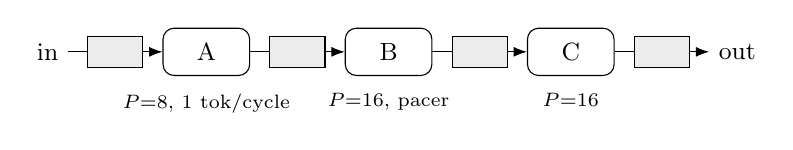
\begin{tikzpicture}[node distance=12mm, every node/.style={font=\small},
  n/.style={draw, rounded corners, minimum width=11mm, minimum height=6mm},
  f/.style={draw, minimum width=7mm, minimum height=4mm, fill=gray!15}]
\node (in) {in};
\node[n, right=of in] (A) {A};
\node[n, right=of A] (B) {B};
\node[n, right=of B] (C) {C};
\node[right=of C] (out) {out};
\foreach \a/\b in {in/A, A/B, B/C, C/out} \draw[-Latex] (\a) -- node[f]{} (\b);
\node[below=1mm of A, font=\scriptsize, align=center] {$P{=}8$, 1 tok/cycle};
\node[below=1mm of B, font=\scriptsize, align=center] {$P{=}16$, pacer};
\node[below=1mm of C, font=\scriptsize, align=center] {$P{=}16$};
\end{tikzpicture}
\end{center}

TAVs ($\NF=8$): A reads and writes at cycles $0..7$ ($P=8$); B reads at
$0,2,\dots,14$ and writes a burst at $8..15$ ($P=16$); C reads and writes at
$0,2,\dots,14$ ($P=16$). As cumulative rows, B's input is
\code{[1 1 2 2 3 3 \dots\ 16 16]} and its output
\code{[0 0 0 0 0 0 0 0 1 2 \dots\ 8 8 8 8 8 8 8 8 8 9 \dots\ 16]}. $\Tg=16$; B and
C are pacers ($16\ge 15.92$), A drives the pacer. Table~\ref{tab:e1} is the
schedule of the pass without causal/latency rules (pass FF).

\begin{table}[h]
\centering\small
\caption{E1, pass FF: wall-clock token times. The input is paced at $\Tg/\NF=2$
cycles per token. A, B and C are stalled until their first input arrives:
A's local cycle 0 runs at cycle 2, B's at 2, C's at 10.}\label{tab:e1}
\begin{tabular}{@{}l*{16}{r}@{}}
\toprule
token $k$ & 1&2&3&4&5&6&7&8&9&10&11&12&13&14&15&16\\
\midrule
input $\to$ A ($w=r$) & 2&4&6&8&10&12&14&16&18&20&22&24&26&28&30&32\\
A $\to$ B, write & 2&4&6&8&10&12&14&16&18&20&22&24&26&28&30&32\\
A $\to$ B, read  & 2&4&6&8&10&12&14&16&18&20&22&24&26&28&30&32\\
B $\to$ C, write & 10&11&12&13&14&15&16&17&26&27&28&29&30&31&32&33\\
B $\to$ C, read  & 10&12&14&16&18&20&22&24&26&28&30&32&34&36&38&40\\
\bottomrule
\end{tabular}
\end{table}

A is input-bound and never runs ahead of B, so \code{A -> B} never holds a token
(peak 0). B writes 8 tokens in 8 cycles while C reads one every 2 cycles: at
cycle 17, 8 tokens are written and 4 read (Figure~\ref{fig:e1}). With the latency
passes every write moves by 32 cycles per node (B's clock starts at 34, C's at
74), which changes no difference between a write and its read on a chain: all four
passes give \code{A -> B} 0 and \code{B -> C} 4; the written depths are 2 and 4,
and 5 on the graph input and output.

\begin{figure}[h]
\centering
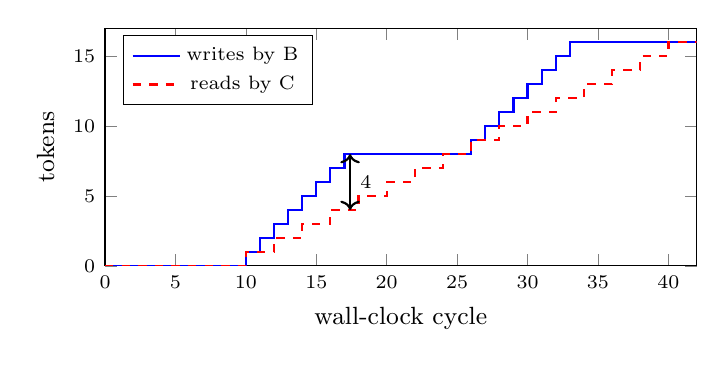
\begin{tikzpicture}
\begin{axis}[width=0.75\textwidth, height=4.6cm, xmin=0, xmax=42, ymin=0, ymax=17,
  xlabel={wall-clock cycle}, ylabel={tokens}, legend pos=north west,
  legend style={font=\scriptsize}, tick label style={font=\scriptsize}, label style={font=\small}]
\addplot[const plot, thick, blue] coordinates {(0,0) (10,1) (11,2) (12,3) (13,4) (14,5) (15,6) (16,7) (17,8) (26,9) (27,10) (28,11) (29,12) (30,13) (31,14) (32,15) (33,16) (42,16)};
\addplot[const plot, thick, red, dashed] coordinates {(0,0) (10,1) (12,2) (14,3) (16,4) (18,5) (20,6) (22,7) (24,8) (26,9) (28,10) (30,11) (32,12) (34,13) (36,14) (38,15) (40,16) (42,16)};
\draw[<->, thick] (axis cs:17.4,4) -- node[right, font=\scriptsize]{4} (axis cs:17.4,8);
\legend{writes by B, reads by C}
\end{axis}
\end{tikzpicture}
\caption{E1, edge \code{B -> C}: cumulative writes and reads (pass FF). The
occupancy is the vertical distance, at most 4 in each frame.}\label{fig:e1}
\end{figure}

%======================================================================
\section{Peak occupancy}\label{sec:peak}
%======================================================================

\begin{lstlisting}[firstnumber=306,title={\texttt{src/finn/transformation/fpgadataflow/derive\_characteristic.py}, lines 306--351}]
def periodic_peak(w, r, period):
    """Peak steady-state occupancy of one frame's schedules repeated every
    ``period`` cycles::

        occ(t) = sum over f of g(t - f*period),   g(u) = |w <= u| - |r <= u|

    ``g`` has finite support, so the sum is finite, and occupancy only changes
    at an event, so event times modulo ``period`` are the only candidates.
    """
    w = np.sort(np.asarray(w, dtype=np.int64))
    r = np.sort(np.asarray(r, dtype=np.int64))
    lo = int(min(w[0], r[0]))
    hi = int(max(w[-1], r[-1]))
    # how many periods of history can still be in flight
    reps = int((hi - lo) // period) + 2
    cand = np.unique(np.concatenate([w, r]) % period) + lo - (lo % period)
    cand = np.concatenate([cand, cand + period])
    occ = np.zeros(len(cand), dtype=np.int64)
    for k in range(reps):
        u = cand + k * period
        occ += np.searchsorted(w, u, side="right") - np.searchsorted(r, u, side="right")
    return int(max(0, occ.max()))


def peak_occupancy(write_times, read_times, period, per_frame, fill_only):
    """Peak occupancy of an edge in steady state.

    The schedules hold two frames. When ``per_frame`` splits them cleanly,
    each frame is evaluated on its own: the first (fill) frame carries the
    pipeline-filling transient and the latency difference a join has to buffer;
    the second (steady) frame carries a producer's run-ahead. Chain edges take
    the larger; ``fill_only`` edges (joins, reconvergent branches) take the
    fill frame alone.
    """
    n = min(len(write_times), len(read_times))
    if n == 0:
        return 0
    w = np.sort(np.asarray(write_times[:n], dtype=np.int64))
    r = np.sort(np.asarray(read_times[:n], dtype=np.int64))
    if per_frame and 2 * per_frame <= n:
        fill = periodic_peak(w[:per_frame], r[:per_frame], period)
        if fill_only:
            return fill
        steady = periodic_peak(w[n - per_frame : n], r[n - per_frame : n], period)
        return max(fill, steady)
    return periodic_peak(w, r, period)
\end{lstlisting}

\paragraph{\code{periodic\_peak}.} Let $g(u)=|\{k: w_k\le u\}|-|\{k: r_k\le u\}|$
be the occupancy of one unit of tokens (one frame) with nothing before or after it.
In steady state a new unit starts every $\Tg$ cycles, so the occupancy is
$\mathrm{occ}(t)=\sum_{f} g(t-f\Tg)$. $g$ has finite support $[\mathrm{lo},\mathrm{hi}]$,
so \code{reps} $=\lfloor(\mathrm{hi}-\mathrm{lo})/\Tg\rfloor+2$ copies suffice
(line 320), and the occupancy only changes at an event, so the event times modulo
$\Tg$ (shifted into the period of lo, and one period later) are the only candidate
phases (321--322). Lines 324--326 add up the copies at each candidate.

\paragraph{\code{peak\_occupancy}: two-frame split (rule R2).} The two stored
frames are evaluated separately whenever the consumer's per-frame token count
splits them cleanly: the \emph{fill} frame (tokens $1..\NF$) carries the
pipeline-filling transient and the latency difference a join has to buffer; the
\emph{steady} frame (the last $\NF$ tokens) carries a producer's run-ahead built
up over the first frame. Chain edges take $\max(\text{fill},\text{steady})$;
\code{fill\_only} edges (joins, reconvergent branches) take the fill frame
alone. If the frames do not split, both are evaluated as one unit. Because that
unit holds two frames but is repeated every \emph{one} period, the joint
evaluation superposes two frames at every instant; on every example edge below it
is exactly twice the per-frame peak (E1 \code{B -> C}: fill 4, steady 4, joint
8; U5 shortcut: fill 449, steady 448, joint 897).

Examples of the split: in E5 (Section~\ref{sec:refill}, with U) the chain edge
\code{U -> A} has fill 0 and steady 2 and takes 2; in E6
(Section~\ref{sec:join}) the branch edge \code{F -> M} has fill 0 and steady 1
and, being \code{fill\_only}, takes 0; in E8c (Section~\ref{sec:causal}) the
shortcut has fill 3 and steady 1 in the causal pass (the causal hold only
acts on the first frame).

%======================================================================
\section{From peak to depth: the rules}\label{sec:rules}
%======================================================================

\subsection{\code{size\_edge} and \code{edge\_depth}}

\begin{lstlisting}[firstnumber=894,title={\texttt{src/finn/transformation/fpgadataflow/derive\_characteristic.py}, lines 894--932}]
    def upstream_cover(tensor):
        """Cycles of supply the FIFOs above ``tensor``'s producer hold while it
        is blocked (they are full then), ``depth * global_period / per_frame``
        each, back along a single-input chain to a pacer, a join or the input."""
        cover = 0.0
        node = model.find_producer(tensor)
        while node is not None and own_period.get(node.name, 0) < pacer_period:
            ins = [t for t in node.input if t in edges]
            if len(ins) != 1:
                break
            t = ins[0]
            cover += max(depths.get(t, 0), 2) * global_period / float(edges[t].per_frame)
            node = model.find_producer(t)
        return int(cover)

    def chain_above(tensor):
        """Slowest period between the last pacer and ``tensor``'s producer
        (the producer excluded)."""
        producer = model.find_producer(tensor)
        return max([edges[t].t_prop for t in producer.input if t in edges], default=0)

    def size_edge(tensor, peak, read_times, consumer, fill_only, idle_floor=0):
        # a write gap is harmless for as long as the consumer's own slack and
        # the supply buffered above the producer last
        slack = max(0, global_period - own_period.get(consumer.name, global_period))
        slack += upstream_cover(tensor)
        depths[tensor] = edge_depth(
            peak,
            read_times,
            edges[tensor],
            fill_only,
            not drives_pacer.get(consumer.name, True),
            global_period,
            pacer_period,
            idle_floor,
            refill_floor(edges[tensor].writes, read_times, slack),
            chain_above(tensor),
            t_down.get(consumer.name, global_period),
        )
\end{lstlisting}
\begin{lstlisting}[firstnumber=826,title={\texttt{src/finn/transformation/fpgadataflow/derive\_characteristic.py}, lines 826--850}]
    if fill_only:
        return max(int(peak), int(idle_floor))
    t_chain = edge.t_up if throttleable else edge.t_full
    allowance = edge.per_frame * (1.0 - min(t_chain, global_period) / float(global_period))
    after_slack = int(round(peak - allowance))
    floor = min(peak, burst_above_rate(read_times, edge.per_frame / float(global_period)))
    if not throttleable:
        floor = max(floor, min(peak, refill))
    # slow stages on both sides of the edge stall each other behind a capped FIFO
    t_pair = t_above + (global_period if t_below is None else t_below)
    if (
        throttleable
        and edge.t_up < pacer_period
        and not (peak > 0 and allowance < CAP_MARGIN * peak)
        and t_pair <= CAP_MARGIN * global_period
    ):
        floor = min(floor, THROTTLED_CAP)
    if (
        throttleable
        and t_below is not None
        and CAP_MARGIN * t_above >= (CAP_MARGIN - 1) * global_period
        and t_above + t_below <= CAP_MARGIN * global_period
    ):
        floor = 0
    return max(after_slack, floor)
\end{lstlisting}

With $\rho=\NF/\Tg$ the edge's average token rate, \code{edge\_depth} computes, for an
edge that is not \code{fill\_only},
\begin{align*}
t_{\mathrm{chain}} &= \begin{cases} t_{\mathrm{up}} & \text{consumer throttleable}\\ t_{\mathrm{full}} & \text{consumer drives the pacer}\end{cases}
\qquad
\mathit{allowance} = \NF\Bigl(1-\frac{\min(t_{\mathrm{chain}},\Tg)}{\Tg}\Bigr)\\
\mathit{after\_slack} &= \mathrm{round}(\mathit{peak}-\mathit{allowance})\\
\mathit{floor} &= \begin{cases}\min(\mathit{peak},\mathit{burst}) & \text{throttleable}\\
  \max\bigl(\min(\mathit{peak},\mathit{burst}),\ \min(\mathit{peak},\mathit{refill})\bigr) & \text{drives the pacer}\end{cases}\\
\mathit{floor} &\leftarrow \min(\mathit{floor}, 256)\quad\text{if throttleable},\ t_{\mathrm{up}}<\Tp,\ \neg(\mathit{peak}>0\wedge \mathit{allowance}<1.25\,\mathit{peak}),\\
  &\qquad\qquad\text{and }t_{\mathrm{above}}+t_{\mathrm{below}}\le1.25\,\Tg\\
\mathit{floor} &\leftarrow 0\quad\text{if throttleable},\ 1.25\,t_{\mathrm{above}}\ge0.25\,\Tg,\ t_{\mathrm{above}}+t_{\mathrm{below}}\le1.25\,\Tg\\
\mathit{depth} &= \max(\mathit{after\_slack},\ \mathit{floor})
\end{align*}
and for a \code{fill\_only} edge $\mathit{depth}=\max(\mathit{peak},\mathit{idle\_floor})$.
$\mathit{burst}$ is \code{burst\_above\_rate(reads}, $\rho$\code{)}, $\mathit{refill}$
is \code{refill\_floor(writes, reads, slack)}, $t_{\mathrm{above}}$ is
\code{chain\_above(tensor)} and $t_{\mathrm{below}}$ the consumer's
\code{downstream\_periods} entry (both passed by \code{size\_edge}; 1.25 is
\code{CAP\_MARGIN}, $0.25/1.25=1-1/\code{CAP\_MARGIN}$). The rules can be grouped as
\emph{depth-minimizing} (R1 paced input, R2 split, R3 relaxation, R7 cap, R7b
decoupled chain) and
\emph{throughput-protecting} (R5 burst floor, R6 refill floor, R4 pacer-bound
chains, R8 joins/branches, R9 idle window, R10 absorbed frame, the cap margin,
the join floor), with R11--R13 correcting the schedule itself.

\subsection{R1 Paced graph input}

\emph{What}: the graph input delivers one frame per $\Tg$, evenly spaced (listing in
Section~\ref{sec:schedule}). \emph{Why}: with an infinitely fast source every
node above the pacer runs ahead, and the edges in front of the pacer grow with the
number of frames considered; a source matched to the accelerator's rate is the
steady state the design must sustain. (\code{fifo\_sizing\_heuristics.rst} reports that on cnv-w1a1 the edge
\code{StreamingDataWidthConverter\_rtl\_0 -> ConvolutionInputGenerator\_rtl\_0} is 60 deep
with the rule and 638 without, at the same rtlsim throughput.)

\emph{Example} (E1 with \code{graph\_input\_schedule} replaced by ``all tokens at
cycle 0''): A then writes at cycles $0..15$ while B reads at $0,2,\dots,30$. On
\code{A -> B} the fill frame peaks at 4, the steady frame at 8 (A has finished
both frames by cycle 15), so the peak is 8; B drives the pacer, $t_{\mathrm{full}}=P_A=8$, the
allowance is $8(1-8/16)=4$, and the depth becomes $\mathrm{round}(8-4)=4$
instead of 2. \code{B -> C} stays 4.

\subsection{R3 Slack relaxation and the reset past the pacer}\label{sec:relax}

\emph{What}: \code{edge\_depth} gives up $\mathit{allowance}=\NF(1-t_{\mathrm{chain}}/\Tg)$
tokens of the peak. \emph{Why}: the peak is the depth at which the producer never
waits, more than throughput needs. A producer whose chain finishes a frame in
$t_{\mathrm{chain}}<\Tg$ cycles can be blocked for $\Tg-t_{\mathrm{chain}}$ cycles a
frame and still deliver on time, and draining $k$ tokens costs $k\Tg/\NF$ cycles.
Past a pacer $t_{\mathrm{prop}}=0$ restarts the chain, so an edge two hops below a
pacer is limited only by the segment since the pacer.

\emph{Example E2}: in $\to$ P $\to$ X $\to$ C, $\Tg=32$. P (pacer, $P=32$) reads
one token every 4 cycles and writes its 8 tokens as a burst in cycles $24..31$;
X ($P=8$) forwards one token a cycle; C reads one token every $k$ cycles. C is not
a pacer and feeds nothing, so it is throttleable. Pass TT schedule (latency
included):
\begin{center}\small
\begin{tabular}{@{}lll@{}}
\toprule
& frame 1 & frame 2\\
\midrule
\code{X -> C} writes & $92..99$ & $124..131$\\
C reads, $k=3$ ($P_C=24$) & $92,95,\dots,113$ & $124,127,\dots,145$\\
C reads, $k=2$ ($P_C=16$) & $92,94,\dots,106$ & $124,126,\dots,138$\\
\bottomrule
\end{tabular}
\end{center}
\begin{center}\small
\begin{tabular}{@{}lrrrrrrrrr@{}}
\toprule
edge & peak & $t_{\mathrm{up}}$ & $t_{\mathrm{full}}$ & allowance & after\_slack & burst & cap & depth & written\\
\midrule
\code{P -> X} & 0 & 32 & 32 & 0 & 0 & 6 & no & 0 & 2\\
\code{X -> C}, $k=3$ & 5 & 8 & 32 & 6.00 & $-1$ & 2 & no & 2 & 2\\
\code{X -> C}, $k=2$ & 4 & 8 & 32 & 6.00 & $-2$ & 4 & yes & 4 & 4\\
\bottomrule
\end{tabular}
\end{center}
For $k=3$ the relaxation takes the depth from the peak 5 to the burst floor 2.
Without the reset past the pacer the edge would carry $t_{\mathrm{up}}=32$, the
allowance would be 0, and \code{edge\_depth} (called with that edge record) returns 5
($k=3$) and 4 ($k=2$). \code{P -> X} is directly below the pacer
($t_{\mathrm{up}}=P_P=32$): no allowance.

\subsection{R4 Pacer-bound chains and the pacer tolerance}\label{sec:pacerbound}

\emph{What}: if the consumer drives the pacer, the relaxation uses
$t_{\mathrm{full}}$ (never reset): below a pacer, $t_{\mathrm{full}}=\Tg$ and the
allowance is 0. \emph{Why}: a chain below a pacer is input-bound at $\Tg$, however
fast its nodes are; once blocked it cannot catch up, and the block propagates to
the pacer through the shallow FIFOs in between. The run-ahead the peak contains
is what carries a consumer that cannot be throttled.

\emph{Example E4}: E2 with C at the pacer's rate (one read every 4 cycles,
$P_C=32$). \code{X -> C}: writes $92..99$, reads $92,96,\dots,120$; peak 6,
$t_{\mathrm{up}}=8$, $t_{\mathrm{full}}=32$, C drives the pacer, so the allowance is 0
and the depth is 6. With \code{pacer\_drivers} replaced so that C is throttleable,
$t_{\mathrm{chain}}=8$, the allowance is 6 and the edge gets 2.

\emph{R4b, pacer tolerance} (\code{PACER\_TOLERANCE}=0.995). \emph{Example E4b}:
the same chain at $\Tg=400$ (P reads every 50 cycles and writes its burst at
$392..399$; C reads every 49 cycles, $P_C=399$). C counts as a pacer ($399\ge398$):
\code{X -> C} has peak 7, allowance 0, depth 7. With an exact test
(\code{PACER\_TOLERANCE}=1.0) C is throttleable, the allowance is
$8(1-8/400)=7.84$ and the depth 2. (Per the \code{.rst}, on mobilenet\_v1 the exact test moves the pacer and the
total depth goes from 9432 to 64586.)

\subsection{R5 Burst floor}

\begin{lstlisting}[firstnumber=561,title={\texttt{src/finn/transformation/fpgadataflow/derive\_characteristic.py}, lines 561--567}]
def burst_above_rate(read_times, rate):
    """Largest excursion of demand above a constant supply ``rate``:
    ``max over t1 < t2 of C(t2) - C(t1) - rate * (t2 - t1)``."""
    if len(read_times) == 0 or rate <= 0:
        return 0
    g = np.arange(1, len(read_times) + 1) - rate * read_times
    return int(np.ceil(np.max(g - np.minimum.accumulate(g))))
\end{lstlisting}

\emph{What}: the depth never falls below $\min(\mathit{peak}, \mathit{burst})$ (except
on a decoupled chain, R7b, and up to the cap of R7) with
$\mathit{burst}=\lceil\max_{k_1\le k_2}\,(k_2-k_1)-\rho\,(r_{k_2}-r_{k_1})\rceil$, the
consumer's largest demand above the edge's average rate line. \emph{Why}: the
relaxation is average-rate arithmetic; a consumer that reads in bursts (an MVAU
reading \code{SF} words at the start of each output window, a sliding-window
generator reading rows) needs its burst buffered even when the average rate is
matched.

\emph{Example} (E2, $k=2$): C reads 8 tokens in 14 cycles against
$\rho=8/32=0.25$: $7-0.25\cdot14=3.5$, so $\mathit{burst}=4$, and the depth is 4. With
\code{burst\_above\_rate} returning 0 the edge gets 2. For $k=3$:
$7-0.25\cdot21=1.75\to2$. Real graph (U1, \code{test\_chained\_tav\_mlp\_chain}):
\code{StreamingDataWidthConverter\_rtl\_0 -> MVAU\_hls\_1} gets 4 from pass FF, where its
peak 4 is held by the burst floor 4 against an allowance of 257.

\subsection{R6 Refill floor and upstream cover}\label{sec:refill}

\begin{lstlisting}[firstnumber=765,title={\texttt{src/finn/transformation/fpgadataflow/derive\_characteristic.py}, lines 765--780}]
def refill_floor(write_times, read_times, slack):
    """Largest number of tokens the consumer reads while the producer writes
    nothing (e.g. while a sliding window generator upstream refills its rows at
    a frame boundary), not counting the first ``slack`` cycles of each gap,
    which are covered otherwise."""
    n = min(len(write_times), len(read_times))
    if n < 2:
        return 0
    w = np.sort(np.asarray(write_times[:n], dtype=np.int64))
    r = np.sort(np.asarray(read_times[:n], dtype=np.int64))
    start, end = w[:-1] + int(slack), w[1:]
    ok = end > start
    if not ok.any():
        return 0
    got = np.searchsorted(r, end[ok], side="left") - np.searchsorted(r, start[ok], side="right")
    return int(max(0, got.max()))
\end{lstlisting}

\emph{What}: for a consumer that drives the pacer, the depth never falls below
$\min(\mathit{peak},\mathit{refill})$: the most tokens the consumer reads during
one gap between consecutive writes, not counting the first \code{slack} cycles of
the gap. \code{slack} (lines 918--919) is the consumer's own slack
$\max(0,\Tg-P_{\mathrm{cons}})$ plus \code{upstream\_cover}: for each FIFO on the
single-input chain above the producer, up to a pacer, a join or the graph input,
$\max(\mathit{depth},2)\cdot\Tg/\NF$ cycles of supply (those FIFOs are full while the
producer is blocked). \emph{Why}: the relaxation removes the producer's run-ahead,
so it delivers just in time; where its writes pause (a sliding-window generator
re-reading rows at a frame boundary), the FIFO alone has to feed the consumer
through the pause.

\emph{Example E5}: in $\to$ A $\to$ C, $\Tg=32$. A ($P=16$) reads 8 tokens in cycles
$0..7$ and then writes 8 in $8..15$ (a window node); C (pacer) reads one token every 4
cycles. Pass TT: \code{A -> C} writes $65..72$ and $97..104$, reads
$65,69,\dots,93$ and $97,\dots,125$; peak 6; $t_{\mathrm{full}}=P_A=16$ (nothing above A
has a period), so the allowance is $8(1-16/32)=4$ and $\mathit{after\_slack}=2$. The largest
write gap is $(72,97)$; with slack 0 (C is the pacer, A's only input is the graph
input) C reads 6 tokens in it ($73,77,\dots,93$): refill 6, depth 6. Without the
rule: 2.

\emph{With an upstream FIFO} (in $\to$ U $\to$ A $\to$ C, U forwarding one token a
cycle): \code{U -> A} is sized first (depth 2), so the cover is $2\cdot32/8=8$
cycles, slack 8; only the reads in $(104+8,129)$ count: $113,117,121,125$, refill 4,
depth 4 (without the rule 2). In E4b the cover is $2\cdot400/8=100$ cycles
(slack $=1+100$).

\subsection{R7 Throttled cap, cap margin and the pair test}

\emph{What}: the floor (burst floor only, for throttleable consumers) is capped at
\code{THROTTLED\_CAP}=256, the SRL depth limit, when the consumer is throttleable,
the producer can be blocked ($t_{\mathrm{up}}<\Tp$), the allowance is not
marginal ($\mathit{allowance}\ge1.25\,\mathit{peak}$, \code{CAP\_MARGIN}) and the
slow stages around the edge fit in \code{CAP\_MARGIN} periods together
($t_{\mathrm{above}}+t_{\mathrm{below}}\le1.25\,\Tg$, the \emph{pair test}).
$\mathit{after\_slack}$ is not capped. \emph{Why}: a throttleable consumer needs
only short-timescale smoothing; it may finish its frame later, so it never has to
hold a frame of run-ahead. The margin: an allowance that only just covers the peak is a
first-order estimate that should not also remove the floor. The pair test: the cap
blocks the producer during the consumer's bursts and so spends the chain's blocking
budget, which the relaxation of the edges further down the same chain spends again;
with a slow stage on each side of the edge nothing is left to absorb the stall, the
two stages stall each other and the pacer loses time. (Per the \code{.rst}: on cnv-w2a2
small, \code{Pool\_hls\_0 -> ConvolutionInputGenerator\_rtl\_3}, peak and burst floor
307, was capped at 256 between stages at 0.88 and 0.91 of the period, and stitched-IP
rtlsim reached 0.980 of the estimate; with the pair test the edge keeps 307 and
reaches 1.000.)

\emph{Example E3}: E2 scaled to $\NF=1024$, $\Tg=4096$ (P writes its frame as a
burst at the end, X forwards, C reads every second cycle, $P_C=2048$).
\code{X -> C}: peak 512, $\mathit{burst}=512$; X is fed by the pacer, so
$t_{\mathrm{above}}=0$, $t_{\mathrm{below}}=P_C$ and the pair test passes.
\begin{center}\small
\begin{tabular}{@{}lrrrrrr@{}}
\toprule
$P_X$ & allowance & $1.25\cdot$peak & cap & depth & without cap & without margin\\
\midrule
1024 & 768 & 640 & yes & 256 & 512 & 256\\
1600 & 624 & 640 & no  & 512 & 512 & 256\\
\bottomrule
\end{tabular}
\end{center}
(``Without margin'' is the tracer's decomposition with the margin condition removed and
the pair test kept: setting \code{CAP\_MARGIN}=0 would also fail the pair test.)

\emph{With a slow node above X} (in $\to$ P $\to$ S $\to$ X $\to$ C, $P_X=1024$; S reads
its frame at one token every one or two cycles and writes it as a burst at the end of
its period $P_S$, so $t_{\mathrm{above}}=t_{\mathrm{up}}=P_S$ on \code{X -> C}; peak and
burst 512 in every row). The last column is the rule of the earlier revision
(\code{39dac9a18}: no pair test, no R7b):
\begin{center}\small
\begin{tabular}{@{}rrrrrlr@{}}
\toprule
$P_S$ & $P_C$ & allowance & $t_{\mathrm{above}}+t_{\mathrm{below}}$ & depth & by & without pair test, R7b\\
\midrule
1024 & 2048 & 768    & 3072 & 2   & R7b & 256\\
2048 & 2048 & 512    & 4096 & 2   & R7b & 512\\
1229 & 4055 & 716.75 & 5284 & 512 & pair test & 256\\
\bottomrule
\end{tabular}
\end{center}
In the last row C still reads every second cycle but has a period of $0.99\,\Tg$: the
two slow stages (0.30 and 0.99 of the period) exceed $1.25\,\Tg$, the cap no longer
applies, and the edge keeps its burst floor 512.

\subsection{R7b Decoupled chain}\label{sec:decoupled}

\emph{What}: no burst floor (and so no cap) for an edge whose consumer is throttleable,
when the slowest node between the last pacer and the producer takes at least
$1-1/\code{CAP\_MARGIN}=20\,\%$ of the period ($t_{\mathrm{above}}\ge0.2\,\Tg$) and the
pair test passes ($t_{\mathrm{above}}+t_{\mathrm{below}}\le1.25\,\Tg$). The depth is then
$\mathit{after\_slack}$, at least 2. \emph{Why}: the burst floor puts the peak back
wherever a consumer reads in bursts against the frame rate, which on a chain of fast
nodes between slow ones is every edge: each fast producer runs a row ahead of the slow
node below it. Behind a shallow FIFO the slow stage above the producer and the slow
stage below the consumer are coupled; at worst they take turns, so a frame takes
$t_{\mathrm{above}}+t_{\mathrm{below}}$, and up to \code{CAP\_MARGIN} periods of that are
taken as harmless. A slow stage above the producer also means the producer is not fed
just in time by the pacer, so blocking it does not stall the pacer at once. Below a
pacer with only fast nodes in between ($t_{\mathrm{above}}<0.2\,\Tg$) the floor stays:
the producer holds the pacer's continuous output while the nodes below pause. (Per the
\code{.rst}: mobilenet\_v1 on the committed U55C folding goes from 97.2 to 17.0~kB of
FIFOs at an unchanged stitched-IP rtlsim interval of 788544 cycles;
\code{test\_fifosizing\_linear[cnv]}, two \code{MVAU\_hls} at 0.67 of the period, is
the case the pair test protects: \code{StreamingDataWidthConverter\_rtl\_12 ->
MVAU\_hls\_7} keeps 63, at 20 rtlsim dropped to 0.83 of the estimate.)

Since every period is at most $\Tg$, the pair test can only fail when
$t_{\mathrm{above}}>0.25\,\Tg$, where the first condition of R7b holds. Together, for
a throttleable consumer: with $t_{\mathrm{above}}<0.2\,\Tg$ the cap of R7 applies as
before; otherwise the burst floor is dropped if the pair fits in $1.25\,\Tg$ and kept
uncapped if it does not.

\emph{Example E3b}: in $\to$ P $\to$ S $\to$ X $\to$ C, $\Tg=32$: E2 with $k=2$
(C reads every 2 cycles, $P_C=16$) and a node S between P and X that reads its 8 tokens
one a cycle ($P_S=8$) or every second cycle and writes them as a burst at the end of its
period $P_S$.
Pass TT for $P_S=16$: \code{X -> C} writes $132..139$, reads $132,134,\dots,146$; peak 4,
burst 4, $t_{\mathrm{up}}=16$, allowance $8(1-16/32)=4$, $\mathit{after\_slack}=0$.
\begin{center}\small
\begin{tabular}{@{}rrrrrr@{}}
\toprule
$P_S$ & $t_{\mathrm{above}}$ & $t_{\mathrm{above}}+t_{\mathrm{below}}$ & decoupled & written & without pair test, R7b\\
\midrule
-- (E2) & 0  & 16 & no (fed by the pacer) & 4 & 4\\
8       & 8  & 24 & yes & 2 & 4\\
16      & 16 & 32 & yes & 2 & 4\\
28      & 28 & 44 & no (pair test) & 4 & 4\\
\bottomrule
\end{tabular}
\end{center}
In E2 the producer X sits directly below the pacer and keeps its burst floor; with a
slow S above it the floor is dropped as long as S and C together fit in
$1.25\cdot32=40$ cycles. For $P_S=16$ the edge \code{P -> S} itself (S is
throttleable, fed by the pacer, $t_{\mathrm{above}}=0$) keeps its peak 4.

\subsection{R8 Joins and reconvergent branches are never relaxed}\label{sec:join}

\emph{What}: \code{fill\_only} edges get $\max(\mathit{peak}_{\mathrm{fill}},\mathit{idle\_floor})$; no
allowance, no burst/refill floor, no cap. \emph{Why}: every relaxation assumes the
consumer can be made to wait. Throttling the early input of a join throttles the
fork it comes from, which starves the other branch---the one the join is waiting
for. A shortcut shallower than the long branch's occupancy deadlocks.

\emph{Example E6}: in $\to$ P0 $\to$ F $\to$ (shortcut $|$ M) $\to$ J, $\Tg=64$.
P0 (pacer) reads and writes one token every 8 cycles; M ($P=16$) reads its 8 tokens in
cycles $0..7$ and writes them in $8..15$; F (\code{DuplicateStreams\_hls}) and J
(\code{ElementwiseAdd\_hls}) are transparent. M is in the branch; \code{F -> M},
\code{F -> J} (the shortcut) and \code{M -> J} are \code{fill\_only}.

\begin{center}
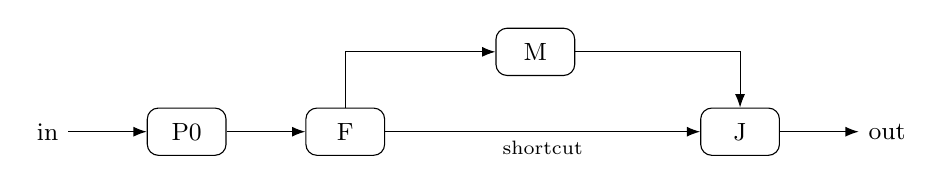
\begin{tikzpicture}[node distance=10mm, every node/.style={font=\small},
  n/.style={draw, rounded corners, minimum width=10mm, minimum height=6mm}]
\node (in) {in};
\node[n, right=of in] (P) {P0};
\node[n, right=of P] (F) {F};
\node[n, above right=4mm and 14mm of F] (M) {M};
\node[n, right=40mm of F] (J) {J};
\node[right=of J] (out) {out};
\draw[-Latex] (in) -- (P); \draw[-Latex] (P) -- (F);
\draw[-Latex] (F) -- node[below, font=\scriptsize]{shortcut} (J);
\draw[-Latex] (F) |- (M); \draw[-Latex] (M) -| (J); \draw[-Latex] (J) -- (out);
\end{tikzpicture}
\end{center}

Pass TT: P0 writes $40,48,\dots,96$ and $104,\dots,160$ (8-cycle input pace, plus 32
cycles latency); F hands this schedule to both branches; M reads it as it arrives,
its writes fall at $97..104$ on its clock and leave at $129..136$ after its own 32-cycle
latency (frame 2: $193..200$). J reads token $k$ at $\max(w^{\mathrm{short}}_k,w^{\mathrm{M}}_k)$, i.e.\ at M's write times.

\begin{center}\small
\begin{tabular}{@{}lrrrrrr@{}}
\toprule
edge & fill & steady & idle floor & depth & as a chain edge & written\\
\midrule
\code{P0 -> F} (chain) & 0 & 0 & -- & 0 & -- & 2\\
\code{F -> M} (branch) & 0 & 1 & 4 & 4 & 0 & 4\\
\code{F -> J} (shortcut) & 12 & 12 & 0 & 12 & 7 & 12\\
\code{M -> J} & 0 & 0 & 0 & 0 & 0 & 2\\
\bottomrule
\end{tabular}
\end{center}

The shortcut holds the whole fill frame (written by cycle 96, read from 129 on)
plus the 4 tokens of the next frame written while M's latency runs out
(Table~\ref{tab:passes}: 8 without latency). Called as a chain edge, \code{edge\_depth}
would give $t_{\mathrm{up}}=0$ (F is fed by a pacer, has no period), allowance 8,
$\mathit{after\_slack}=4$, burst floor 7: depth 7 instead of 12.

\subsection{R9 Idle-window floor}

\begin{lstlisting}[firstnumber=728,title={\texttt{src/finn/transformation/fpgadataflow/derive\_characteristic.py}, lines 728--744}]
def idle_window_floor(curve, throttleable):
    """Tokens that arrive while the consumer is not reading this stream: a
    frame's tokens times the fraction of the consumer's period spent outside
    its read window. Zero for continuous readers. Capped for a consumer that
    can be throttled through its idle window instead."""
    half = len(curve) // 2
    if half < 2:
        return 0
    per_frame = int(curve[half - 1])
    if per_frame <= 0:
        return 0
    reads = np.searchsorted(curve, np.arange(1, per_frame + 1), side="left")
    duty = min(1.0, float(reads[-1] - reads[0] + 1) / float(half))
    want = int(round(per_frame * (1.0 - duty)))
    if throttleable:
        want = min(want, THROTTLED_CAP)
    return want
\end{lstlisting}

\emph{What}: for \code{fill\_only} edges into a characterized consumer, the
depth is at least the frame's tokens times the fraction of the consumer's period
outside its read window (first to last read of the stream, from the consumer's own TAV),
capped at 256 for a throttleable consumer. It is computed for every characterized consumer
(line 985) but only used by \code{fill\_only} edges. \emph{Why}: inside a branch the
consumer cannot be made to wait, so whatever the producer delivers while the
consumer is not reading must be buffered (\code{FMPadding} emits padding without
reading; an MVAU reads a short burst per output window).
\emph{Example} (E6, \code{F -> M}): M reads in 8 of its 16 cycles, duty $0.5$,
$\mathrm{round}(8\cdot0.5)=4$: depth 4 instead of its fill peak 0; with
\code{idle\_window\_floor} returning 0 the edge gets 2.

\subsection{R10 Absorbed-frame floor}

\begin{lstlisting}[firstnumber=747,title={\texttt{src/finn/transformation/fpgadataflow/derive\_characteristic.py}, lines 747--762}]
def absorbed_frame_floor(node, tensor):
    """One folded input frame, for a consumer whose TAV reads nothing in the
    stored window (a node that absorbs its whole input frame before releasing
    anything, e.g. a FINNLoop)."""
    cons = registry.getCustomOp(node)
    try:
        idx = list(node.input).index(tensor)
        shape = cons.get_folded_input_shape(idx)
    except Exception:
        return 0
    if shape is None or len(shape) < 2:
        return 0
    n = 1
    for d in shape[:-1]:
        n *= int(d)
    return int(n)
\end{lstlisting}

\emph{What}: a consumer whose TAV reads nothing on an input in the stored window
gets one folded input frame (product of the folded input shape without the last
dimension) on that edge. \emph{Why}: a node that absorbs a whole frame before releasing
anything (a \code{FINNLoop} body) may be characterized in a window that misses the
absorb phase; there is no schedule to compare against. \emph{Example E7}: in $\to$ A $\to$ L,
L's input TAV is all zeros, L is an MVAU with 8 input vectors of one word: \code{A -> L}
gets 8 (\code{absorbed=8}), without any peak computation.

\subsection{R11 Phase lead}\label{sec:lead}

\begin{lstlisting}[firstnumber=354,title={\texttt{src/finn/transformation/fpgadataflow/derive\_characteristic.py}, lines 354--367}]
def phase_lead(out_curve, in_curves):
    """Output tokens a TAV writes before its first read on any streamed input.

    The stored window can begin inside a frame: an MVAU_rtl emits a feature
    map's outputs during the next feature map's window, after it prefetched the
    inputs, so its TAV opens with ``MH / PE`` writes whose reads lie before the
    window. Those tokens belong to the previous frame.
    """
    firsts = [int(np.argmax(np.asarray(c) > 0)) for c in in_curves if int(c[-1]) > 0]
    if not firsts or min(firsts) == 0:
        return 0
    if frame_tokens(out_curve) > sum(frame_tokens(c) for c in in_curves):
        return 0  # an expanding node may write before reading (e.g. FMPadding)
    return int(out_curve[min(firsts) - 1])
\end{lstlisting}

\emph{What}: the output tokens a TAV writes before its first read on any input
belong to the previous frame; in the causal passes the output tokens are renumbered
past them (lines 392--394 of \code{causal\_writes}, below). Not applied to a node that writes
more words than it reads per frame (an \code{FMPadding} legitimately writes first).
\emph{Why}: the stored window can begin inside a frame; an \code{MVAU\_rtl} emits
a feature map's outputs during the next window, after prefetching its inputs, so taken
at face value its outputs precede the inputs that carry them and every such node in a
branch looks one feature map faster.

\emph{Function level} (unit test): output row \code{[1 2 2 2 3 3 4 5 5 5 6 6]}, input row
\code{[0 0 1 2 3 3 3 3 4 5 6 6]}: first read in cycle 2, lead $=$ out[1] $=2$
(0 if the output is doubled, an expanding node). \code{causal\_writes(writes=[0 10
\dots\ 70], lead=2)} returns \code{[20 30 40 50 60 70 80 90]}: tokens 3.. become
1.., and the last two are tokens 1--2 of the next frame shifted by one frame span.

\emph{Example E8d}: E6's residual with $\Tg=32$ and a one-to-one branch node M
($P=10$) that writes at cycles $0..7$ but reads at $2..9$ (lead 2). Pass FF:
M writes tokens 1 and 2 at cycles 0 and 1, before P0 has delivered anything, and J
reads the shortcut as fast as it arrives: shortcut peak 0. Pass TF: M's writes are
renumbered to \code{[4 8 12 16 20 24 33 34 | 36 \dots\ 56 65 66]}, J now waits for M's
7th and 8th token until cycles 33, 34, and the shortcut needs 2. With latency:
6 (FT) against 10 (TT). Final depth 10. Real graph (U3,
\code{test\_chained\_tav\_residual\_mvau\_rtl}, two \code{MVAU\_rtl} with lead 31 in
the branch): shortcut 27 / 28 in passes FF / FT, 88 / 90 in TF / TT.

\subsection{R12 Causal writes}\label{sec:causal}

\begin{lstlisting}[firstnumber=370,title={\texttt{src/finn/transformation/fpgadataflow/derive\_characteristic.py}, lines 370--402}]
def causal_writes(write_times, in_scheds, lead=0):
    """Hold each output token of the first frame until the inputs that carry it
    have arrived.

    A TAV has an arbitrary phase, so its ``first_write - first_read`` is not the
    node's latency: a 64:1 width converter measures as writing one cycle after
    its first read. With ``N_in`` inputs and ``N_out`` outputs a frame, output
    *j* cannot precede input ``ceil((j+1) * N_in / N_out)``. Only applied over
    the first frame (where the pipeline starts empty) and only to compacting
    nodes (``N_in > N_out``).

    The ``lead`` tokens written before the first read (``phase_lead``) belong
    to the previous frame: the output tokens are renumbered past them, in every
    frame, and the last ``lead`` are placed one frame after the first ones.
    """
    if not in_scheds:
        return write_times
    n_out = len(write_times)
    if n_out == 0:
        return write_times
    out = np.array(write_times, dtype=np.int64, copy=True)
    fill = max(1, n_out // 2)  # a TAV stores two frames
    if 0 < lead < fill and n_out > fill:
        span = out[n_out - 1] - out[n_out - 1 - fill]
        out = np.concatenate([out[lead:], out[fill : fill + lead] + span])
    idx = np.arange(1, fill + 1, dtype=np.int64)
    for sched, _ in in_scheds.values():
        n_in = len(sched)
        if n_in == 0 or n_in <= n_out:
            continue  # expanding or one-to-one: the clock already covers it
        need = np.minimum(-(-idx * (n_in // 2) // fill), n_in)
        out[:fill] = np.maximum(out[:fill], sched[need - 1])
    return np.maximum.accumulate(out)
\end{lstlisting}

\emph{What} (causal passes): with $N_{\mathrm{in}}$ input and $N_{\mathrm{out}}$ output
tokens per frame, output token $j$ ($1$-based) of the \emph{first} frame is held until
input token $\lceil j N_{\mathrm{in}}/N_{\mathrm{out}}\rceil$ has arrived, for every
input with $N_{\mathrm{in}}>N_{\mathrm{out}}$ (compacting); then the schedule is made
monotone. \emph{Why}: a TAV's first-write-minus-first-read is not the node's latency;
a 64:1 width converter measured by rtlsim writes one cycle after its first read,
which would let its consumer start before the tokens it needs can exist.

\emph{Function level}: a 4:1 compactor, inputs at $0,10,\dots,150$, TAV writes all
at 0: held to \code{[30 70 70 70]} (inputs 4 and 8; the second frame is only made
monotone). \emph{In a chain} (E8b: in $\to$ P $\to$ K $\to$ C, K reads 8 and writes 2
at its cycles 1 and 5): K's writes \code{[8 24 40 56]} become \code{[16 32 40 56]}; the
depths do not change (a chain moves together). Note that the second-frame token at 40
still precedes its 4th input (48): the hold is first-frame only.

\emph{In a branch} (E8c: P0 $\to$ F $\to$ (shortcut $|$ K $\to$ E) $\to$ J with K as above and E
expanding 2 to 8): shortcut 1 (FF) / 17 (FT) without, 3 (TF) / 19 (TT) with the hold;
written 19. In pass TF the fill frame peaks at 3 and the steady frame at 1.

\subsection{R13 Node latency and block writes}

\begin{lstlisting}[firstnumber=521,title={\texttt{src/finn/transformation/fpgadataflow/derive\_characteristic.py}, lines 521--558}]
def block_writes(write_times, node, in_scheds):
    """Hold output word *j* until the input block it belongs to is complete,
    for the inputs a node consumes in whole blocks (``tav_input_blocks``):
    word *j* needs the first ``(j // out_words + 1) * in_words`` words of that
    input. Applied over both frames; held words leave at most one per cycle.

    A dynamic ``MVAU`` computes on the matrix ``dynamic_load`` buffered from
    in1, but its TAV reads in1 alongside the compute.
    """
    try:
        blocks = tav_input_blocks(registry.getCustomOp(node))
    except Exception:
        return write_times
    out = np.array(write_times, dtype=np.int64, copy=True)
    j = np.arange(len(out), dtype=np.int64)
    held = False
    for idx, (in_words, out_words) in blocks.items():
        if idx >= len(node.input) or node.input[idx] not in in_scheds:
            continue
        sched = in_scheds[node.input[idx]][0]
        if len(sched) == 0 or in_words < 1 or out_words < 1:
            continue
        need = np.minimum((j // out_words + 1) * in_words, len(sched))
        out = np.maximum(out, sched[need - 1])
        held = True
    if not held:
        return write_times
    return np.maximum.accumulate(out - j) + j


def node_latency(node):
    """Cycles a node's writes trail its TAV: ``TAV_PIPELINE_LATENCY`` plus the
    node's own ``tav_extra_latency`` (e.g. an ``InnerShuffle`` page)."""
    try:
        extra = int(tav_extra_latency(registry.getCustomOp(node)))
    except Exception:
        extra = 0
    return TAV_PIPELINE_LATENCY + max(0, extra)
\end{lstlisting}

\emph{What} (latency passes): every characterized node's writes are delayed by
\code{TAV\_PIPELINE\_LATENCY}$=32$ cycles plus \code{tav\_extra\_latency(inst)}
(0 for every op except \code{InnerShuffle}: one page, $I J/\mathrm{SIMD}$ cycles). In the causal-and-latency
pass, writes are also held to whole input blocks of \code{tav\_input\_blocks(inst)}
(none except a dynamic MVAU's in1: the whole $MW\cdot MH/PE$-word matrix for its
$\mathit{numInputVectors}[-1]\cdot MH/PE$ outputs), with held words leaving at most one per
cycle. \emph{Why}: a TAV contains no latency. On a chain that does not matter (E1);
where two paths meet the slower path's latency is what the early input buffers.
32 is deliberately above the rtlsim-measured latencies listed in the code comment (1 to 69 cycles).

Both per-node quantities are module functions of \file{} that dispatch on the op
class (\code{isinstance}); the custom ops carry no sizer hooks (until commit
\code{30960c3d1} they were \code{HWCustomOp} methods \code{get\_tav\_extra\_latency} and
\code{get\_tav\_input\_blocks}, overridden by \code{InnerShuffle} and \code{MVAU}):

\begin{lstlisting}[firstnumber=405,title={\texttt{src/finn/transformation/fpgadataflow/derive\_characteristic.py}, lines 405--429}]
def tav_extra_latency(inst):
    """Cycles from the arrival of an input word to the first output word that
    depends on it, beyond ``TAV_PIPELINE_LATENCY``. A TAV records the steady
    state at an arbitrary phase and cannot show it. An ``InnerShuffle``
    transposes a page in a bank: none of its words leaves before all
    ``I * J / SIMD`` of them are in, at most one per cycle."""
    if isinstance(inst, InnerShuffle):
        in_shape = inst.get_nodeattr("transpose_in_shape")
        return int(in_shape[-2]) * int(in_shape[-1]) // inst.get_nodeattr("SIMD")
    return 0


def tav_input_blocks(inst):
    """``{input index: (in_words, out_words)}`` for the inputs a node consumes
    in whole blocks, block *b* of ``out_words`` output words needing block *b*
    of ``in_words`` words of that input complete. A dynamic ``MVAU`` computes on
    the matrix its ``dynamic_load`` buffered from in1: the
    ``numInputVectors[-1] * MH / PE`` outputs of a matrix need all
    ``MW * MH / PE`` words of it."""
    if isinstance(inst, MVAU) and inst.get_nodeattr("mem_mode") == "dynamic":
        n_reps = inst.get_nodeattr("numInputVectors")[-1]
        nf = inst.get_nodeattr("MH") // inst.get_nodeattr("PE")
        burst = inst.get_nodeattr("MW") * inst.get_nodeattr("MH") // inst.get_nodeattr("PE")
        return {1: (burst, n_reps * nf)}
    return {}
\end{lstlisting}

\emph{Examples}: E6, shortcut 8 without and 12 with latency: M's 32 cycles at
$\rho=8/64$ are 4 tokens. U5 (\code{test\_chained\_tav\_residual\_latency}: two DWCs and four
\code{MVAU\_rtl} at SIMD $=$ PE $=32$ in the branch, below a 515-cycle pacer): shortcut 262 without, 449 with latency
(about $6\cdot32\cdot512/515$ tokens more). Function level (unit test): a dynamic
\code{MVAU\_rtl} with $MW{=}4$, $MH{=}2$, $PE{=}1$, 3 vectors (\code{tav\_input\_blocks}
$=\{1:(8,6)\}$), matrix words at $0,10,\dots,150$, TAV writes $0..11$: held to
\code{[70 71 72 73 74 75 150 151 152 153 154 155]}; an \code{InnerShuffle\_rtl} with a
$16\times8$ page at SIMD 2 has \code{node\_latency} $=32+64=96$.

\subsection{Width converters}\label{sec:dwc}

There is no DWC-specific rule in the sizer. DWCs are inserted before
characterization and carry tree-model TAVs fixed by the width ratio
(\code{StreamingDataWidthConverter.get\_tree\_model}: down-conversion reads one word every
\code{writes\_per\_read} cycles and writes every cycle; up-conversion reads every
cycle and writes on the cycle the last input word arrives). They interact with the
rules in three places: (i) an up-converting (narrow-to-wide) DWC is a compacting
node, so R12 applies to it (it is the motivating case for R12 with rtlsim TAVs);
(ii) its window $(N_{\mathrm{in}},N_{\mathrm{out}})$ in lowest terms is used by the join floor (a 48:1 DWC needs 48
fork words per output word, Section~\ref{sec:joinfloor}); (iii) its burst pattern drives
the burst floor of the next edge (U1: \code{StreamingDataWidthConverter\_rtl\_0 ->
MVAU\_hls\_1}, depth 4). With tree-model TAVs the hold is a no-op: in U6
(\code{MVAU\_hls} PE 2 $\to$ 4:1 DWC $\to$ \code{MVAU\_hls} SIMD 8) the DWC's first output in
pass TF is at cycle 272, the arrival of its 4th input word, before and after the hold. In U5 the two DWCs
of the branch (512 to 16 words and back) are ordinary branch nodes (\code{fill\_only}).

%======================================================================
\section{The four passes and how they are combined}\label{sec:passes}
%======================================================================

\code{DeriveFIFOSizes} runs the complete chained pass four times (listing in
Section~\ref{sec:overview}): without/with \emph{causal} (R11 phase-lead renumbering and R12 hold of
the first frame) and without/with \emph{latency} (R13 delay; with both, also R13 block
writes). Each pass is a complete, independent schedule derivation; the only state
is the model. The result per edge is the \emph{maximum} over the four passes. The
reasoning in the code: each variant is a lower bound on the requirement under a
different modelling error. Without the hold a producer's run-ahead survives (the
TAV may let it write early); with it a compacting node shows its real latency. The
latency lengthens the slower path into a join, but can also shift and smooth a
burst so that a floor disappears. Table~\ref{tab:passes} shows each case.

\begin{table}[h]
\centering\small
\caption{Depth per pass (before the minimum of 2) and the written depth. F/T: causal, latency off/on;
DWC: \code{StreamingDataWidthConverter}.}\label{tab:passes}
\begin{tabular}{@{}llrrrrrl@{}}
\toprule
graph & edge & FF & FT & TF & TT & written & largest from\\
\midrule
E6 & \code{F -> J} (shortcut) & 8 & 12 & 8 & 12 & 12 & latency\\
E8c & \code{F -> J} (shortcut) & 1 & 17 & 3 & 19 & 19 & causal + latency\\
E8d & \code{F -> J} (shortcut) & 0 & 6 & 2 & 10 & 10 & causal + latency\\
E8d & \code{M -> J} & 2 & 2 & 0 & 0 & 2 & --\\
U1 & \code{DWC\_rtl\_0 -> MVAU\_hls\_1} & 4 & 0 & 0 & 0 & 4 & neither\\
U1 & \code{MVAU\_hls\_0 -> DWC\_rtl\_0} & 1 & 0 & 0 & 0 & 2 & --\\
U3 & \code{DuplicateStreams -> ElementwiseAdd} & 27 & 28 & 88 & 90 & 90 & causal + latency\\
U3 & \code{MVAU\_rtl\_2 -> ElementwiseAdd} & 7 & 7 & 0 & 0 & 7 & non-causal\\
U5 & \code{DuplicateStreams -> ElementwiseAdd} & 262 & 449 & 262 & 449 & 449 & latency\\
\bottomrule
\end{tabular}
\end{table}

In U1 only pass FF gives the DWC edge a nonzero depth (peak 4, kept by the burst
floor): there the tree-model TAVs of \code{MVAU\_hls\_0} and of the DWC both write a
token before their first read, the DWC writes 5 words in cycles $0..4$ and
\code{MVAU\_hls\_1} reads one of them and the other 4 only after a pause of its own
TAV. In the causal passes \code{MVAU\_hls\_0}'s lead token is renumbered into the
previous frame, in the latency passes the 32-cycle delays stall \code{MVAU\_hls\_1}
long enough to absorb its pause (the code comment: latency ``can also smooth a pacer's
read bursts''); both give 0, and the max keeps 4. U3's
\code{MVAU\_rtl\_2 -> ElementwiseAdd} likewise keeps its 7 from the non-causal passes.
The max is therefore conservative by construction; the \code{.rst} reports that the
four passes double the sizing time against two (210~s against 108~s on resnet50).

%======================================================================
\section{Join window floor}\label{sec:joinfloor}
%======================================================================

After the passes, every input of a two-stream join (\code{is\_stream\_join}:
\code{AddStreams}, \code{ElementwiseAdd} with two streamed inputs) or of a
\code{StreamingConcat} that reconverges a fork gets a floor that does not come from
any TAV. (Unlike the adds, a concat is characterized, so in the passes it is an ordinary
node whose inputs are \code{fill\_only}.) \emph{Why}: a fork writes all its outputs
together, so it stalls as soon as one branch is full. If the long branch reads many
fork words before its first output reaches the join (a vector of $MW/SIMD$ words for an
MVAU, a softmax row, a DWC window), the other inputs must buffer what the fork writes
meanwhile, or the fork stalls, the long branch never completes its window and the
graph deadlocks. The timeline pass misses this where a TAV writes before it reads
(MVAU tree models) and the fork is transparent, and it does not size a shortcut at
all when the fork is fed directly by the graph input. Where the long branch runs
through padding, sliding windows and upsampling (the C2f, FPN and PAN stages of yolov8,
which meet at concats), each node delays it by rows of its own resolution, a lag the
floor only sees through the per-word input needs below.

\begin{lstlisting}[firstnumber=1074,title={\texttt{src/finn/transformation/fpgadataflow/derive\_characteristic.py}, lines 1074--1081}]
    def input_need(inst, i, k):
        # input words of input i the first k output words need
        table = tav_input_need(inst, i)
        if table is not None:
            frames, j = np.divmod(k - 1, len(table))
            return table[j] + frames * _frame_words(inst, i)
        in_words, out_words = tav_input_window(inst, i)
        return ceil_div(k, out_words) * in_words
\end{lstlisting}
\begin{lstlisting}[firstnumber=1097,title={\texttt{src/finn/transformation/fpgadataflow/derive\_characteristic.py}, lines 1097--1162}]
        def walk(t, m):
            """``(need, times)`` of the first ``m`` tokens on ``t``: the fork
            input words they need and their arrival times. None off the fork."""
            if t in memo and len(memo[t][0]) >= m:
                return memo[t][0][:m], memo[t][1][:m]
            p = producer(t)
            if p is None or p.name in above:
                return None
            inst = registry.getCustomOp(p)
            k = np.arange(1, m + 1, dtype=np.int64)
            o = list(p.output).index(t)
            n_out = _frame_words(inst, o, output=True)
            if p.name == fork.name:
                n_in = _frame_words(inst, 0)
                need = ceil_div(k * n_in, n_out)
                res = need, need * float(period) / n_in
            else:
                need, ready = None, None
                for i, x in enumerate(p.input):
                    if producer(x) is None:
                        continue
                    idx = input_need(inst, i, k)
                    up = walk(x, int(idx[-1]))
                    if up is None:
                        continue
                    n_i, t_i = up[0][idx - 1], up[1][idx - 1]
                    need = n_i if need is None else np.maximum(need, n_i)
                    ready = t_i if ready is None else np.maximum(ready, t_i)
                if need is None:
                    return None
                try:
                    rate = float(inst.get_exp_cycles()) / n_out
                except Exception:
                    rate = 0.0
                res = need, rate * k + np.maximum.accumulate(ready - rate * k)
            memo[t] = res
            return res

        try:
            # join token k: the k-th word of every input of an add, the k-th
            # block of each input's share of a concatenated pixel
            sizes = [
                _frame_words(registry.getCustomOp(join), list(join.input).index(t)) for t in ins
            ]
            n_join = int(np.gcd.reduce(sizes))
            per = [n // n_join for n in sizes]
            k = np.arange(1, 2 * n_join + 1, dtype=np.int64)
            walks = [walk(t, 2 * n) for t, n in zip(ins, sizes)]
        except Exception:
            continue
        if any(w is None for w in walks):
            continue
        total = np.max(np.stack([w[0][k * c - 1] for w, c in zip(walks, per)]), axis=0)
        taken = np.max(np.stack([w[1][k * c - 1] for w, c in zip(walks, per)]), axis=0)
        try:
            rate = float(registry.getCustomOp(join).get_exp_cycles()) / n_join
        except Exception:
            rate = 0.0
        taken = rate * k + np.maximum.accumulate(taken - rate * k)
        for t, (need, times), c in zip(ins, walks, per):
            deadlock = np.searchsorted(need, total - 1, side="right") - (k - 1) * c
            paced = np.searchsorted(times, taken, side="right") - (k - 1) * c
            backlog = int(max(deadlock.max(), paced.max()))
            if backlog > 1:
                floors[t] = int(np.ceil(backlog * (1 + JOIN_FLOOR_MARGIN)))
    return floors
\end{lstlisting}

\begin{description}
\item[Fork and walk.] The fork is the latest common ancestor (in graph order) of all
  join inputs. \code{walk(t, m)} returns, for the first $m$ tokens on tensor $t$, the
  number of fork input words they need ($\mathit{need}$) and their arrival times.
  At the fork, output token $k$ needs $\lceil kN_{\mathrm{in}}/N_{\mathrm{out}}\rceil$ words,
  arriving at $\mathit{need}\cdot\mathit{period}/N_{\mathrm{in}}$ (the fork paced at the graph's
  period). At any other node, \code{input\_need} composes the node's window
  \code{tav\_input\_window(inst, i)} $=(a,b)$ (output block of $b$ words needs the first
  $(\lceil k/b\rceil) a$ input words; \code{MVAU} in0 a vector, $TH$ vectors when tiled;
  \code{HWSoftmax} a row; \code{InnerShuffle} a page; else the blocks of
  \code{tav\_input\_blocks}, else the frame-size ratio in lowest terms) or, for a node
  that reorders a frame, the need of every output word of a frame,
  \code{tav\_input\_need(inst, i)}: \code{FMPadding} (a padding word needs the input up to
  the last real pixel before it), \code{ConvolutionInputGenerator} (a window its last
  pixel), \code{UpsampleNearestNeighbour} (a pixel its nearest neighbour) and
  \code{OuterShuffle} (from its permutation); later frames add one input frame per
  frame. The times follow $T(j)=\max(T_{\mathrm{in}}(\mathit{need}(j)),T(j-1)+r)$
  with $r$ = \code{get\_exp\_cycles()}/$N_{\mathrm{out}}$ (line 1131, as a running maximum).
\item[Join token.] $N_{\mathrm{join}}$ is the greatest common divisor of the input
  frame sizes and input $i$ contributes $c_i=N_i/N_{\mathrm{join}}$ words to a join token
  (lines 1138--1142): an add takes one word of every input, a concat each input's share
  of a pixel (or of a fraction of one). Join token $k$ on input $i$ is its word $k\,c_i$.
\item[Two backlogs] over two join frames ($k=1..2N_{\mathrm{join}}$):
  \emph{deadlock}: to deliver join token $k$ on every input the fork must write
  $W(k)=\max_i \mathit{need}_i(k\,c_i)$ words, so input $i$ holds the words it can make from the
  first $W(k)-1$ fork words minus the $(k-1)c_i$ the join has taken (line 1157);
  \emph{paced}: the join takes token $k$ at the latest input's arrival, no faster
  than its own rate, and input $i$ holds what has arrived by then minus $(k-1)c_i$ (1158).
\item[Floor] $\lceil 1.25\cdot\max(\text{backlogs})\rceil$ (\code{JOIN\_FLOOR\_MARGIN}),
  only if the backlog exceeds 1; it raises the passes' depth, never lowers it.
\end{description}

The input windows and input needs (module functions of \file{}, like those of R13):

\begin{lstlisting}[firstnumber=432,title={\texttt{src/finn/transformation/fpgadataflow/derive\_characteristic.py}, lines 432--463}]
def tav_input_window(inst, ind=0):
    """For the join floor: ``(in_words, out_words)``, output block *b* of
    ``out_words`` words needs the first ``(b + 1) * in_words`` words of input
    ``ind``.

    * ``MVAU``: the ``MH / PE`` outputs of a vector need all ``MW / SIMD``
      words of it; the tiled MVU (TH > 1) computes a group of TH vectors
      together.
    * ``HWSoftmax``: a vector is normalized by its maximum and sum, none of its
      outputs leaves before all of it is in.
    * ``InnerShuffle``: a page leaves only once all of it is in.
    * otherwise the blocks of ``tav_input_blocks``, else the ratio of the folded
      frame sizes in lowest terms (a 48:1 width converter needs 48 words a word,
      a one-to-one node one).
    """
    if isinstance(inst, MVAU) and ind == 0:
        th = inst.get_nodeattr("TH")
        sf = inst.get_nodeattr("MW") // inst.get_nodeattr("SIMD")
        return sf * th, inst.get_nodeattr("MH") // inst.get_nodeattr("PE") * th
    if isinstance(inst, HWSoftmax):
        fold = inst.get_folded_input_shape()[-2]
        return fold, fold
    if isinstance(inst, InnerShuffle):
        page = tav_extra_latency(inst)
        return page, page
    blocks = tav_input_blocks(inst)
    if ind in blocks:
        return blocks[ind]
    n_in = int(np.prod(inst.get_folded_input_shape(ind)[:-1]))
    n_out = int(np.prod(inst.get_folded_output_shape()[:-1]))
    g = np.gcd(n_in, n_out)
    return n_in // g, n_out // g
\end{lstlisting}
\begin{lstlisting}[firstnumber=466,title={\texttt{src/finn/transformation/fpgadataflow/derive\_characteristic.py}, lines 466--518}]
def tav_input_need(inst, ind=0):
    """For the join floor, nodes that reorder a frame: an array over one frame's
    output words, entry *j* the number of words of input ``ind`` output word *j*
    needs. None for every other node (``tav_input_window`` then applies).

    * ``FMPadding``: output word *j* needs the input up to its own pixel, a
      padding word the input up to the last pixel before it.
    * ``ConvolutionInputGenerator``: the words of output pixel (y, x) need the
      input up to the last pixel of its window.
    * ``UpsampleNearestNeighbour``: output pixel (y, x) needs the input up to
      its nearest neighbour.
    * ``OuterShuffle``: output word *j* is input word ``src[j]`` of the
      transposed frame, so it needs the first ``max(src[:j + 1]) + 1`` words
      (only when the innermost dimension, folded by SIMD, stays innermost).
    """
    if isinstance(inst, FMPadding):
        h, w = inst.get_nodeattr("ImgDim")
        top, left = inst.get_nodeattr("Padding")[:2]
        ho, wo = inst.get_padded_odim()
        words = int(np.prod(inst.get_folded_input_shape()[:-1])) // (h * w)
        row, col = np.divmod(np.arange(ho * wo), wo)
        inside = (row >= top) & (row < top + h)
        pixels = np.clip(row - top, 0, h) * w + np.where(inside, np.clip(col - left + 1, 0, w), 0)
        return np.repeat(np.maximum(pixels * words, 1), words)
    if isinstance(inst, ConvolutionInputGenerator):
        h, w = inst.get_nodeattr("IFMDim")
        k_h, k_w = inst.get_nodeattr("ConvKernelDim")
        s_h, s_w = inst.get_nodeattr("Stride")
        d_h, d_w = inst.get_nodeattr("Dilation")
        oshape = inst.get_folded_output_shape()
        oh, ow = oshape[1], oshape[2]
        words_in = int(np.prod(inst.get_folded_input_shape()[:-1])) // (h * w)
        words_out = int(np.prod(oshape[:-1])) // (oh * ow)
        y, x = np.divmod(np.arange(oh * ow), ow)
        last = (y * s_h + (k_h - 1) * d_h) * w + x * s_w + (k_w - 1) * d_w
        return np.repeat((np.minimum(last, h * w - 1) + 1) * words_in, words_out)
    if isinstance(inst, UpsampleNearestNeighbour):
        hi, wi = inst.get_nodeattr("HI"), inst.get_nodeattr("WI")
        ho, wo = inst.get_nodeattr("HO"), inst.get_nodeattr("WO")
        words = inst.get_nodeattr("NumChannels") // inst.get_nodeattr("SIMD")
        b, rest = np.divmod(np.arange(inst.get_nodeattr("batchSize") * ho * wo), ho * wo)
        y, x = np.divmod(rest, wo)
        pixels = b * hi * wi + (y * hi // ho) * wi + x * wi // wo + 1
        return np.repeat(pixels * words, words)
    if isinstance(inst, OuterShuffle):
        perm = list(inst.get_nodeattr("perm"))
        shape = list(inst.get_nodeattr("transpose_in_shape"))
        if perm[-1] != len(perm) - 1:
            return None
        shape[-1] //= inst.get_nodeattr("SIMD")
        src = np.arange(int(np.prod(shape))).reshape(shape).transpose(perm).reshape(-1)
        return np.maximum.accumulate(src) + 1
    return None
\end{lstlisting}

\emph{Example E10} (\code{make\_residual(nvec=2, ch=8, simd=1, pe=1)}, tree-model TAVs,
period 132): fork PE 1 (16 words a frame), MVAU $MW=MH=8$, SIMD=PE=1, window
$(8,8)$, \code{get\_exp\_cycles}=128. The fork is fed by the graph input, so the four passes
size only \code{MVAU -> join} (0).

\begin{center}\small
\begin{tabular}{@{}lrrrrrrrrr@{}}
\toprule
$k$ & 1&2&3&$\cdots$&8&9&10&$\cdots$&16\\
\midrule
shortcut: need, time & 1, 8.2 & 2, 16.5 & 3, 24.8 & & 8, 66.0 & 9, 74.2 & 10, 82.5 & & 16, 132.0\\
MVAU: need, time & 8, 66 & 8, 74 & 8, 82 & & 8, 122 & 16, 132 & 16, 140 & & 16, 188\\
$W(k)$, taken & 8, 66 & 8, 74 & 8, 82 & & 8, 122 & 16, 132 & 16, 140 & & 16, 188\\
shortcut deadlock & 7 & 6 & 5 & & 0 & 7 & 6 & & 0\\
shortcut paced & 8 & 7 & 7 & & 7 & 8 & 7 & & 7\\
\bottomrule
\end{tabular}
\end{center}

The MVAU needs all 8 words of a vector before its first output, so to deliver join token 1
the fork must write 8 words; the shortcut holds the 7 tokens of words $1..7$ (deadlock
backlog 7), and paced, the 8 words that have arrived at cycle 66 when the join takes
token 1 (paced backlog 8). The floor is $\lceil 1.25\cdot8\rceil=10$: written depth of
the shortcut 10 (without the floor 2). The MVAU input has backlog 1 (no floor).
U4 (\code{test\_join\_window\_floor}, $MW=MH=64$, 16 vectors): floor $\lceil1.25\cdot64\rceil=80$.
U3: floor 78, below the passes' 90; U5: floor 40, below 449; E6: floor 3, below 12.

\emph{Example E11} (\code{make\_concat\_window()} of \code{test\_join\_window\_floor\_concat}):
fork \code{DuplicateStreams} (4$\times$4 pixels, 2 channels, PE 1: 32 words a frame)
$\to$ (shortcut $|$ \code{FMPadding} (pad 1, 72 words) $\to$ 3$\times$3
\code{ConvolutionInputGenerator\_rtl} (SIMD 1: 18 words a pixel, 288 a frame)) $\to$
\code{StreamingConcat}. No TAVs; with \code{period=None} the floor takes the largest
\code{get\_exp\_cycles()}, the concat's 320, so the fork writes a word every 10 cycles.
$N_{\mathrm{join}}=\gcd(32,288)=32$: a join token is one shortcut word and 9 window
words, half a pixel. The window of output pixel $(0,0)$ ends at padded pixel $(2,2)$,
\code{FMPadding} word 30, which needs the input up to pixel $(1,1)$: 12 fork words
(\code{tav\_input\_need} of the generator starts \code{[30 \dots]}, of \code{FMPadding}
\code{[1 1 \dots\ 1 2 2 4 4 \dots]}).
\begin{center}\small
\begin{tabular}{@{}lrrrrrrrr@{}}
\toprule
$k$ & 1&2&3&4&5&6&7&8\\
\midrule
$W(k)$ & 12&12&14&14&16&16&16&16\\
taken & 129.8&139.8&149.8&159.8&169.8&179.8&189.8&199.8\\
shortcut deadlock & 11&10&11&10&11&10&9&8\\
shortcut paced & 12&12&12&12&12&12&12&12\\
window input paced & 9&9&9&9&9&9&9&9\\
\bottomrule
\end{tabular}
\end{center}
Floors: shortcut $\lceil1.25\cdot12\rceil=15$, window input $\lceil1.25\cdot9\rceil=12$
(\code{\{'short': 15, 'l2': 12\}}). Before commit \code{2cd2a077d} the concat got no
floor and the three window nodes counted as one-to-one through their frame ratio.
(Per the \code{.rst}: on yolov8\_4w4a small, the PAN concat's shortcut
\code{DuplicateStreams\_hls\_11 -> StreamingConcat\_hls\_12} got 9086 from the timeline
and stitched-IP rtlsim produced no output in 383~M cycles; the floor raises it to
13842, from a structural backlog of 8704 and a paced one of 11073, and the design
completes at 1.000 of the estimate.)

%======================================================================
\section{Writing the depths}\label{sec:write}
%======================================================================

\begin{lstlisting}[firstnumber=1202,title={\texttt{src/finn/transformation/fpgadataflow/derive\_characteristic.py}, lines 1202--1238}]
        # InsertFIFO takes max(producer.outFIFODepths, consumer.inFIFODepths),
        # so depths already on the nodes (e.g. from a folding config) would
        # override the sizer. Reset both, then write both.
        for node in hw_nodes:
            inst = registry.getCustomOp(node)
            inst.set_nodeattr("inFIFODepths", [self.minimum_size] * len(node.input))
            inst.set_nodeattr("outFIFODepths", [self.minimum_size] * len(node.output))

        graph_inputs = [x.name for x in model.graph.input]
        for node in hw_nodes:
            assert not node.op_type.startswith("StreamingFIFO"), "Found existing FIFOs"
            prod = registry.getCustomOp(node)
            out_fifo_depths = []
            for output_name in node.output:
                cons_node = model.find_consumer(output_name)
                if cons_node is None:
                    # graph output
                    out_fifo_depths.append(self.io_fifo_depth)
                    continue
                fifo_depth = max(depths.get(output_name, self.minimum_size), self.minimum_size)
                out_fifo_depths.append(fifo_depth)
                cons = registry.getCustomOp(cons_node)
                in_depths = cons.get_nodeattr("inFIFODepths")
                for i, inp in enumerate(cons_node.input):
                    if inp == output_name:
                        in_depths[i] = fifo_depth
                cons.set_nodeattr("inFIFODepths", in_depths)
            prod.set_nodeattr("outFIFODepths", out_fifo_depths)

            # graph inputs get at least io_fifo_depth
            in_fifo_depths = prod.get_nodeattr("inFIFODepths")
            for i, input_name in enumerate(node.input):
                if input_name in graph_inputs:
                    in_fifo_depths[i] = max(self.io_fifo_depth, in_fifo_depths[i])
            prod.set_nodeattr("inFIFODepths", in_fifo_depths)

        return (model, False)
\end{lstlisting}

\begin{itemize}
\item Existing \code{inFIFODepths}/\code{outFIFODepths} (e.g.\ from a folding
  config) are reset to 2 first, because \code{InsertFIFO} takes the maximum of the
  producer's and the consumer's value and would otherwise override the sizer.
\item Every internal edge gets $\max(\mathit{depth},2)$; edges the passes did not size
  (absent from the dict) get 2. The value is written on both endpoints.
\item A graph output gets exactly \code{io\_fifo\_depth}=5, a graph input
  $\max(5,\cdot)$; their edges are never sized by the timeline (line 978). The
  \code{.rst} notes that this is where the sizer uses more storage than the
  \code{largefifo\_rtlsim} reference on the MLPs (5 instead of 2 on wide input streams).
\item \code{InsertFIFO(create\_shallow\_fifos=True)} then creates a FIFO on every edge.
  If \code{default\_swg\_exception} is set, the builder afterwards applies
  \code{CapConvolutionFIFODepths} (outside \code{DeriveFIFOSizes}): a FIFO between a
  \code{ConvolutionInputGenerator} and an \code{MVAU} is capped to one image row
  ($W\cdot\mathit{ifold}$, rounded by \code{optimize\_depth}).
\end{itemize}

%======================================================================
\section{Summary of the rules}
%======================================================================

\begin{center}\small
\begin{tabular}{@{}p{0.16\textwidth}p{0.23\textwidth}p{0.29\textwidth}p{0.24\textwidth}@{}}
\toprule
rule & where & effect & example\\
\midrule
R1 paced input & \code{graph\_input\_schedule} & input at $\NF/\Tg$ tokens per cycle & E1: 4 $\to$ 2\\
R2 frame split & \code{peak\_occupancy} & fill / steady frame evaluated separately & E1: 8 $\to$ 4\\
R3 relaxation, reset & \code{edge\_depth}, \code{chain\_period} & $-\NF(1-t_{\mathrm{chain}}/\Tg)$ & E2: 5 $\to$ 2\\
R4 pacer-bound & \code{edge\_depth} ($t_{\mathrm{full}}$) & no allowance below a pacer for pacer drivers & E4: 2 $\to$ 6\\
R4b tolerance & \code{PACER\_TOLERANCE} & pacer if $P_v\ge0.995\Tg$ & E4b: 2 $\to$ 7\\
R5 burst floor & \code{burst\_above\_rate} & $\ge\min(\mathit{peak},\mathit{burst})$ & E2: 2 $\to$ 4\\
R6 refill floor, cover & \code{refill\_floor}, \code{upstream\_cover} & $\ge\min(\mathit{peak},\mathit{refill})$, pacer drivers & E5: 2 $\to$ 6 (4 with U)\\
R7 cap, margin, pair & \code{THROTTLED\_CAP}, \code{CAP\_MARGIN} & floor $\le256$ for throttleable, not between slow stages & E3: 512 $\to$ 256; with S: 256 $\to$ 512\\
R7b decoupled chain & \code{chain\_above}, \code{downstream\_periods} & no floor for throttleable below a slow stage & E3b: 4 $\to$ 2\\
R8 join/branch & \code{fill\_only} & fill peak, never relaxed & E6: 7 $\to$ 12\\
R9 idle window & \code{idle\_window\_floor} & branch edges $\ge$ idle share & E6: 2 $\to$ 4\\
R10 absorbed frame & \code{absorbed\_frame\_floor} & one folded frame & E7: 8\\
R11 phase lead & \code{phase\_lead} & renumber lead tokens & E8d: 6 $\to$ 10\\
R12 causal hold & \code{causal\_writes} & first-frame outputs wait for inputs & E8c: 17 $\to$ 19\\
R13 latency, blocks & \code{node\_latency}, \code{block\_writes} & +32 cycles (+ extra), block holds & E6: 8 $\to$ 12\\
passes & \code{DeriveFIFOSizes} & max over 4 variants & U1: 4 kept\\
join floor & \code{join\_window\_floors} & $\ge1.25\cdot$ backlog (adds, concats) & E10: 2 $\to$ 10; E11: 15\\
min / IO & \code{DeriveFIFOSizes} & $\ge2$; IO $=5$ & all\\
\bottomrule
\end{tabular}
\end{center}

%======================================================================
\section{Observations}\label{sec:obs}
%======================================================================

Points where the code's behaviour is not obvious, or where
\code{docs/finn/fifo\_sizing\_heuristics.rst} and the code differ in emphasis:
\begin{enumerate}
\item \textbf{Fork fed by the graph input.} A transparent node with no scheduled input
  is skipped (line 945), so its outputs get no edge: the shortcut and the first edge of
  each branch are not sized by the four passes, and the branch's first node runs
  unstalled (U2, U4, E10). Only the join floor sizes such a shortcut. The \code{.rst}
  mentions this only in its bert example.
\item \textbf{Chains fed by the paced input.} The graph input contributes no period
  to $t_{\mathrm{up}}/t_{\mathrm{full}}$, so above the first pacer $t_{\mathrm{full}}$ is the
  largest node period, below $\Tg$, and edges into pacer drivers get a positive allowance
  although the chain is input-bound at $\Tg$ (E1: allowance 4 on \code{A -> B}). The
  ``pacer-bound chains'' argument of the \code{.rst} (an input-bound chain cannot catch up)
  would apply here too; in practice the paced input keeps these peaks small, and R6 still
  applies.
\item \textbf{Two-frame split.} The \code{.rst} says joint evaluation ``double-counts the
  transient''. In the code the joint unit (two frames) is repeated every single period,
  which doubles any per-frame peak, transient or not (all examples here: joint $=2\times$).
\item \textbf{Idle-window floor scope.} The \code{.rst} says it applies to edges into a node
  inside a reconvergent branch; the code applies it to every \code{fill\_only} edge into a
  characterized consumer, which also includes a characterized node with two produced inputs
  (e.g.\ a dynamic MVAU). Joins (transparent) never get it.
\item \textbf{Tree-model input rows.} With a single-row tree-model TAV and several
  streamed inputs, every input is bound to row 0 (\code{stream\_curves}).
\item \textbf{Stale docstring.} \code{dataflow\_performance(use\_characterized=True)} still
  says fork and join vectors ``are copied from their neighbours''; the \code{.rst} states that
  this rule (\code{inherited\_fork\_join\_tav\_lengths}) was removed, and the code agrees.
\item \textbf{Cap and decoupled chain.} Every period is at most $\Tg$, so the pair test of
  R7 can only fail where $t_{\mathrm{above}}>0.25\,\Tg$, and there the first condition of
  R7b already holds: for a throttleable consumer below a stage of at least $0.2\,\Tg$ the
  burst floor is either dropped (R7b) or kept uncapped, and the cap of R7 only acts with
  $t_{\mathrm{above}}<0.2\,\Tg$. The \code{.rst} describes the two as separate rules.
  $t_{\mathrm{below}}$ includes the consumer's own period and everything below it, also
  the branches of a fork below the consumer.
\item The join floor is called with the caller's period (\code{self.period}), the four
  passes with $\max(\text{caller},\text{TAVs})$; with \code{period=None} the floor falls back to
  the largest \code{get\_exp\_cycles()} (the unit test gets 79 for U3 that way, the builder path 78).
\end{enumerate}

\appendix
%======================================================================
\section{Reproducing the numbers}\label{app:repro}
%======================================================================

All scripts are in \code{claude-tools/finn-examples-features/fifo\_sizing\_writeup/scripts/}
of the \code{claude-tools} branch, run against commit \code{4ce1bd188}. They are pure Python (tree models and hand-made TAVs; no
synthesis, no rtlsim) and run in seconds.
\begin{description}
\item[\code{fifotrace.py}] wraps the module-level functions of \file{} (and a line tracer on
  \code{join\_window\_floors}) for the duration of one \code{DeriveFIFOSizes} call; FINN is not
  modified. It records schedules, peaks (fill / steady / joint) and the terms of
  \code{edge\_depth}, asserting that its decomposition reproduces the returned depth.
\item[\code{fifo\_examples.py}] builds E1--E11 and U1--U6 and prints everything; ablations
  replace one module-level name for one call (the cap margin and the pair test are
  removed in the tracer's decomposition instead, since \code{CAP\_MARGIN} enters both).
\item[\code{run\_examples.sh}] sets up the environment for a worktree:
\begin{lstlisting}[language=bash,numbers=none]
git -C /home/lstasytis/finn worktree add build/wt/pr-fifo \
    feature/dev/analytical-fifo-sizing          # commit 4ce1bd188
claude-tools/finn-examples-features/tools/wtsetup.sh build/wt/pr-fifo
scripts/run_examples.sh /home/lstasytis/finn/build/wt/pr-fifo --all-passes \
    > scripts/fifo_examples_output.txt
python scripts/build_tex.py /home/lstasytis/finn/build/wt/pr-fifo   # listings
\end{lstlisting}
\item[\code{fifo\_examples\_output.txt}] the output this document was written from.
\item[\code{build\_tex.py}, \code{fifo\_sizing\_analytical.tex.in}] produce this file, copying
  every listing verbatim from the source tree.
\end{description}

\end{document}
